\chapter{Le prototype de calorimètre à lecture semi-digitale}
\label{chap.sdhcal}
Dans ce chapitre le prototype de calorimètre à lecture semi-digitale qui a été construit au sein de l’institut de physiques nucléaire de Lyon en 2011 sera décrit. Ce prototype a été testé lors de plusieurs campagnes de test en faisceau au CERN. Pendant ces tests, le prototype a été exposé à un flux de particules tel que des pions, des protons, des muons et des électrons. Nous détaillerons les différents méthodes utilisées pour reconstruire l’énergie des hadrons incidents. 
\minitoc
\newpage

%%%%%%%%%%%%%%%%%%%%%%%%%%%%%%%%%%%%%%%%%%%%%%%

\section{Les gerbes hadroniques}
Lorsqu'un hadron de haute énergie traverse un matériau dense, il interagit avec les noyaux de celui-ci. Cette interaction produit généralement plusieurs particules secondaires qui vont à leur tour interagir avec le milieu et créer d'autres particules. L'ensemble de ces processus constitue une gerbe hadronique.  La gerbe hadronique prend fin lorsque l'énergie des particules filles n'est plus suffisante pour créer des hadrons. Cependant des processus de basse énergie vont continuer jusqu'à l'arrêt ou l'absorption des particules filles. Ce phénomène de gerbe hadronique s'observe dans les expérience de physique de particules où les hadrons créé voyagent jusqu'aux calorimètres. Ils induisent alors ces cascades de particules. L'énergie déposée et mesurée dans les calorimètres permet alors de retrouver l'énergie de la particule incidente. Ce phénomène s'observe aussi dans l'atmosphère lorsqu'un rayon cosmique interagit dans l'atmosphère. Ces rayons cosmiques peuvent être des gammas, des protons, des noyaux d'hélium, des électrons... Les rayons cosmiques sont principalement générés à l'extérieur du système solaire et pourraient avoir comme origine des noyaux actifs de galaxie, l'explosion de supernovas ou des trous noirs. La figure~\ref{fig:cosmicShowerScheme} montre un schéma de développement d'une gerbe hadronique induite par un proton cosmique.
\begin{figure}[!h]
  \begin{center}
    \includegraphics[width=.7\textwidth]{SDHCAL/figs/cosmicShower.jpg}
    \caption{Schéma du développement d'une gerbe hadronique induite par un proton cosmique.}
    \label{fig:cosmicShowerScheme}
  \end{center}
\end{figure}
Ce schéma illustre le nombre important de variétés de particules secondaires pouvant être générer. On peut distinguer deux composantes dans les gerbes hadroniques: une partie électromagnétique et et une non-électromagnétique.\\

La fraction électromagnétique est composée d'électrons et de photons, provenant souvent de la désintégration des mésons neutres $\pi^{0}$ et $\eta$. Les processus mis en jeu dans cette composante sont les suivants:  
\begin{itemize}
\item Le rayonnement Bremsstralung: $e^-~+~noyau~\rightarrow~e^-~+~\gamma$ 
\item La production de paire (pour des photons d'énergie supérieure à $1022\ keV$): $\gamma~+~noyau~\rightarrow~e^+e^-$  
\item L'annihilation: $e^+~+~atome~\rightarrow~2\gamma~+~ion$
\item L'effet Compton: $\gamma~+~atome~\rightarrow~\gamma~+~e^-~+~ion$
\item L'effet photoélectrique (pour des photons de faible énergie): $\gamma~+~atome~\rightarrow~e^-~+~ion$ 
\end{itemize}
La fraction non électromagnétique est plus complexe. En effet, en plus de l’ionisation par les particules chargées, des processus d'interaction faible et forte sont mis en jeu. Des interactions inélastiques des hadrons avec les noyaux du milieu produisent des particules secondaires. Les noyaux sont souvent laissés dans des états excités après ces interactions. Ils retrouvent un état fondamental via des processus de désintégrations et de fragmentations nucléaires. De plus, plusieurs effets induisent des difficultés supplémentaires ou des erreurs pour l'analyse des gerbes hadroniques. D'une part, une fraction de l'énergie hadronique est invisible, à cause de la capture stable de protons ou de neutrons par des noyaux. 
D'autre part, une autre fraction de l'énergie hadronique est détectée avec du retard. En effet, les processus d'interaction faible et forte peuvent entraîner l'émission de neutrons qui ont besoin de se thermaliser pour se lier à un noyau. Ces phénomènes peuvent exciter des noyaux avec un retard par rapport au développement de la gerbe hadronique car la thermalisation des neutrons est un phénomène lent. La désintégration tardive de ces noyaux, peut engendrer une perte d'information pour l’événement ou même du bruit pour les événements suivants. Enfin les muons et les neutrinos émis pendant le développement de la cascade peuvent s'échapper du détecteur. La fraction d'énergie manquante entraînera des difficultés pour la mesure de l'énergie de la particule incidente et dégradera la résolution en énergie du détecteur.
\begin{figure}[!h]
  \begin{center}
    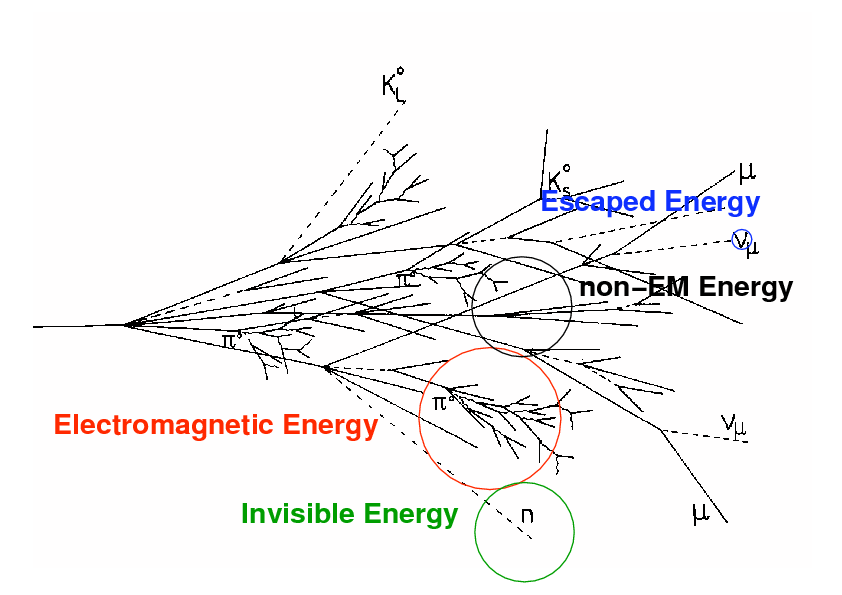
\includegraphics[width=.8\textwidth]{SDHCAL/figs/had-shower.png}
    \caption{Schéma du développement d'une gerbe hadronique.}
    \label{fig:showerScheme}
  \end{center}
\end{figure}
La figure~\ref{fig:showerScheme} montre un schéma de gerbe hadronique. Les différentes composantes de la cascade sont sont mis en évidence.

\textcolor{red}{blabla sur la longueur d'interaction}

%%%%%%%%%%%%%%%%%%%%%%%%%%%%%%%%%%%%%%%%%%%%%%%

\section{Le SDHCAL}
Le calorimètre hadronique à lecture semi-digitale est un concept de calorimètre à échantillonnage développé au sein de la collaboration CALICE. La partie active est composée de chambres à plaques résistives de verre (GRPC). Un prototype de calorimètre à lecture semi-digitale a été construit en 2011 à l’institut de physique nucléaire de Lyon. Les principaux objectifs de ce prototype étaient de montrer qu'un calorimètre gazeux ultra-granulaire peux réaliser des mesures précises de l'énergie de hadrons et de valider l'intérêt de ce type de détecteur pour l'application d'algorithmes de suivi de particules (Paricule Flow Algorithm PFA). Il est composé de 48 chambres à plaques résistives de verre  de 1 $m^2$, insérées dans des cassette en acier de 0.25 $cm$ d'épaisseur qui participe à l'absorbeur. Ces cassettes sont insérées dans une structure autoporteuse en acier construit dans le laboratoire CIEMAT en Espagne. Les cassettes sont alors séparées par des plaques en acier de 1.5 $cm$ d'épaisseur. Ainsi les GRPC du prototypes sont séparées par 2 $cm$ d'acier. La taille du prototype est $1\times1\times1.3~m^3$ et sa profondeur totale correspond à 6$\lambda_I$ ($\lambda_I\simeq20.4~cm$ pour les pions dans le fer). La figure~\ref{fig:proto} est une photographie du prototype sur la ligne de faisceau H6 du SPS (Super Proton Synchrotron) au CERN.
\begin{figure}[!h]
  \begin{center}
    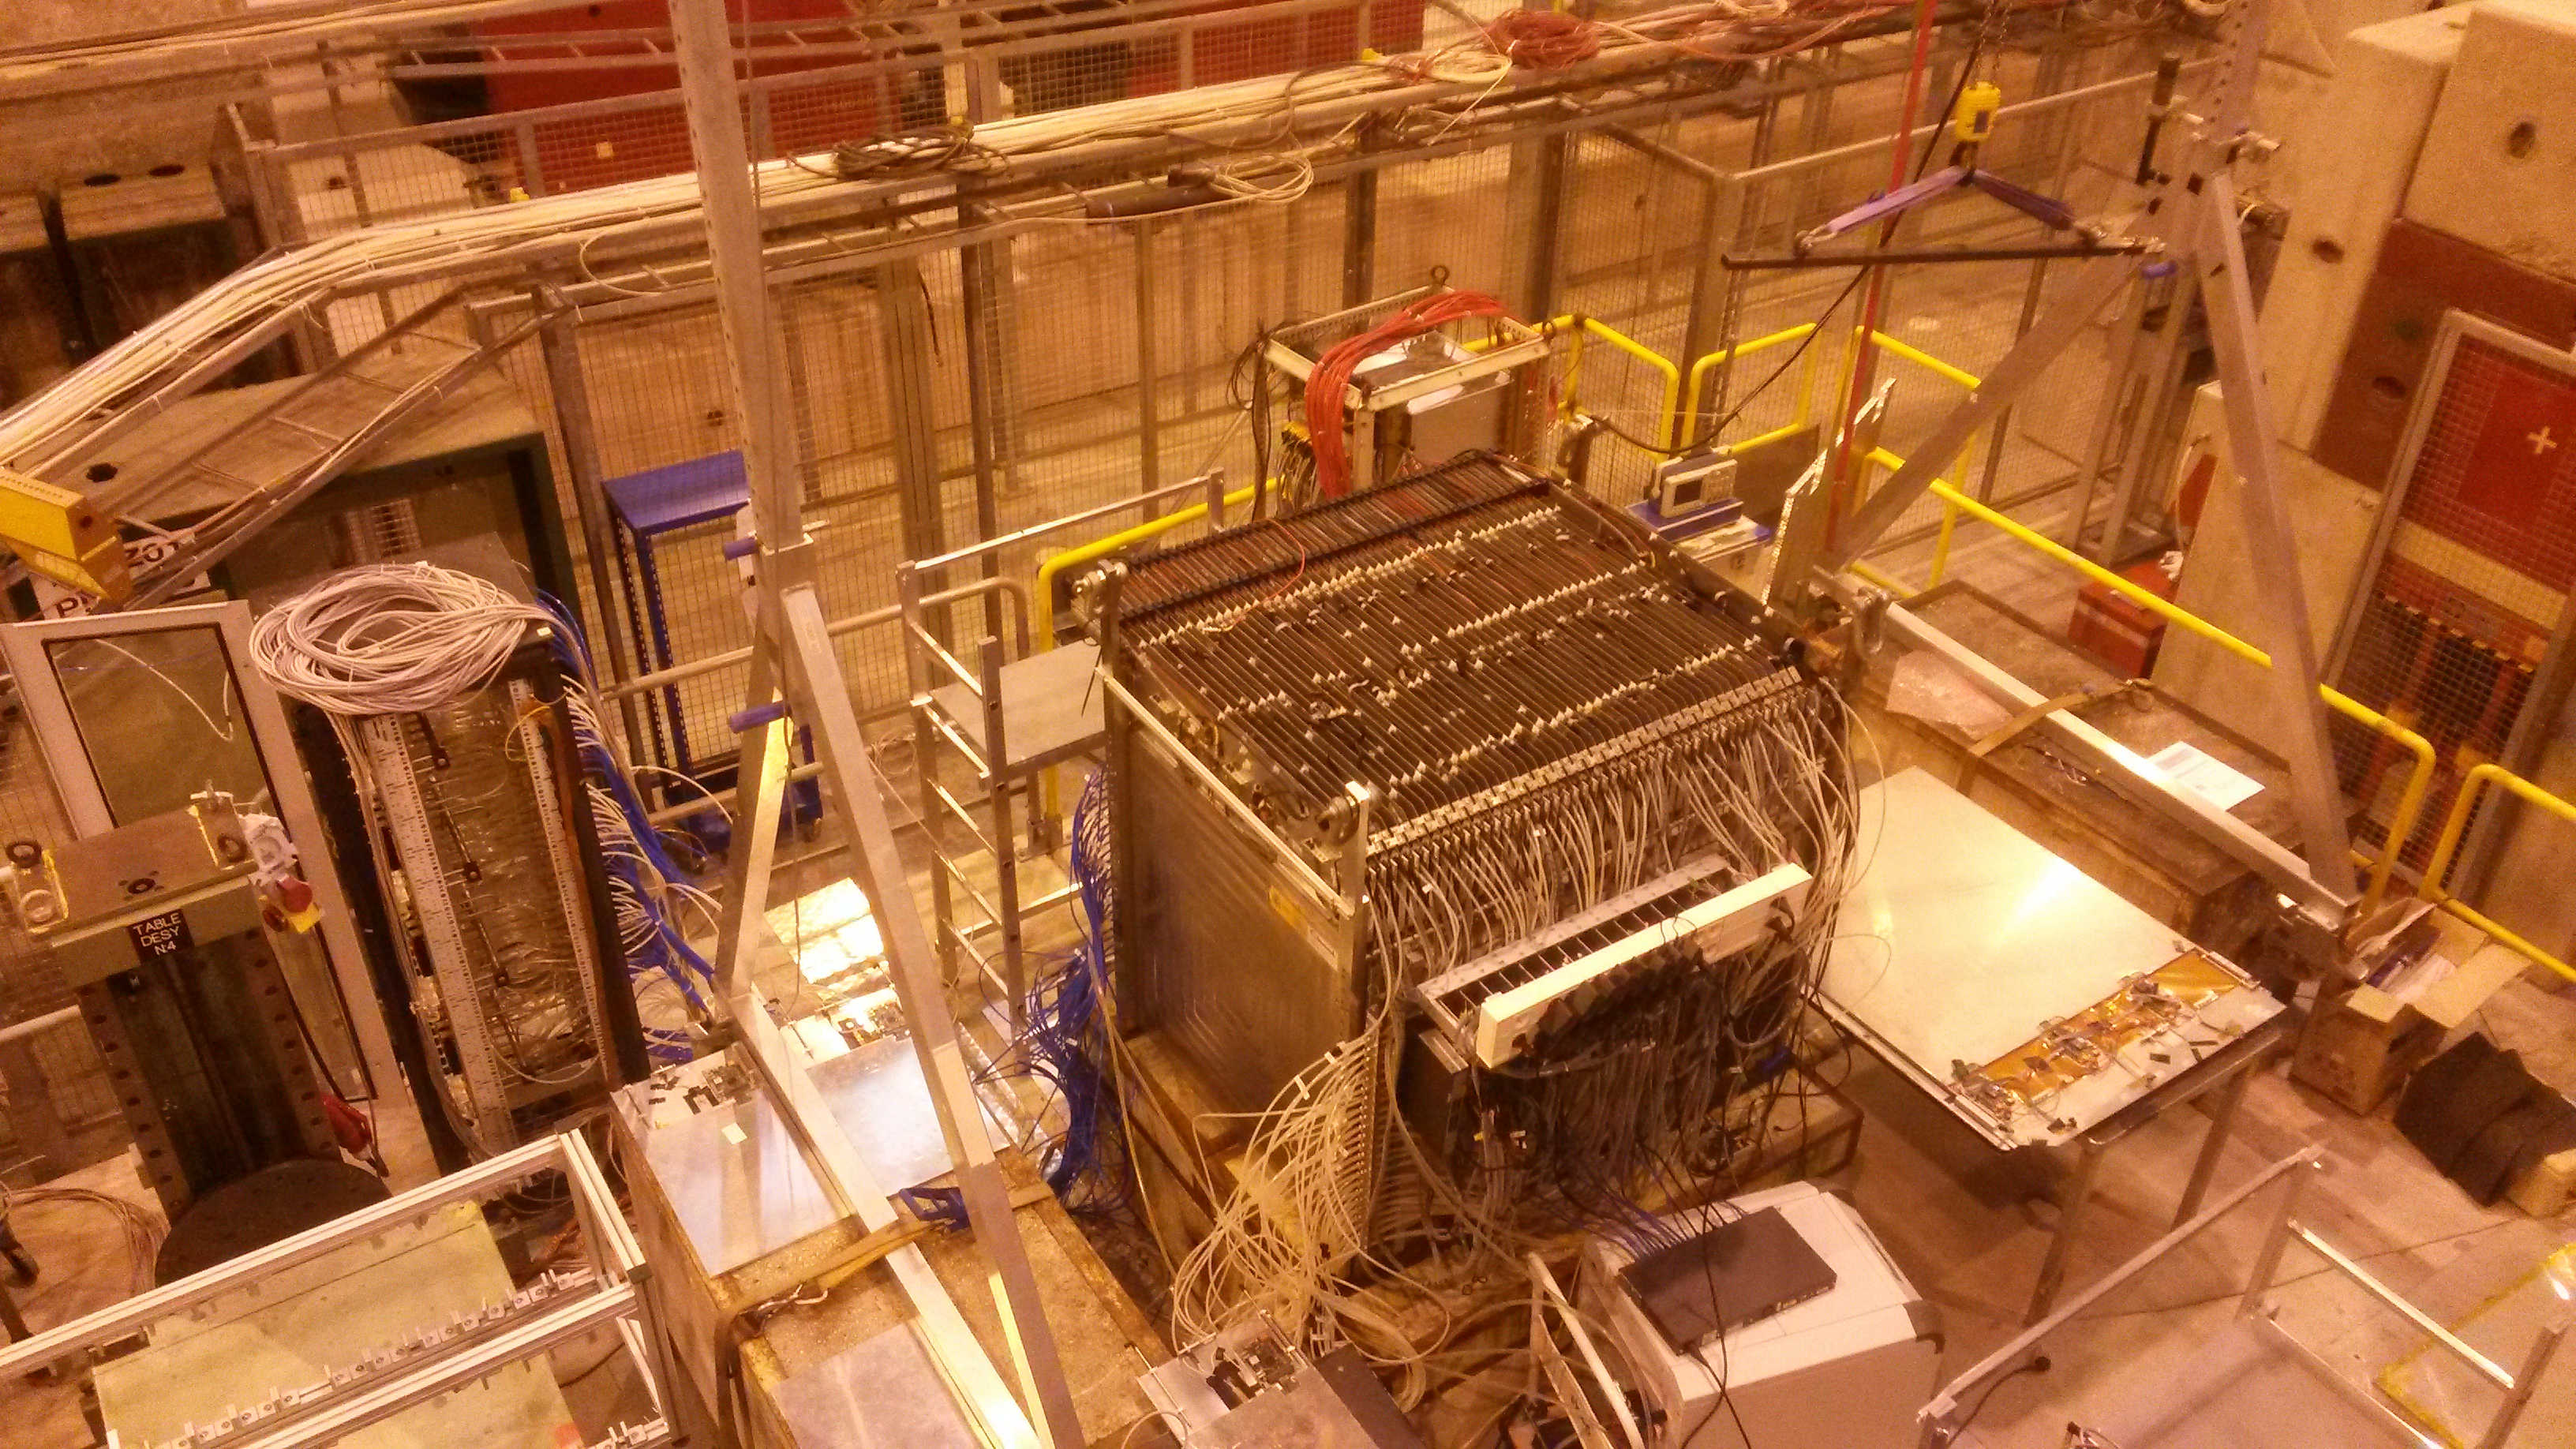
\includegraphics[width=.8\textwidth]{SDHCAL/figs/proto.jpg}
    \caption{Le prototype du calorimètre à lecture semi-digitale sur la ligne de faisceau H6 du CERN.}
    \label{fig:proto}
  \end{center}
\end{figure}
%
Contrairement à la majorité des calorimètres, le SDHCAL n'a pas été optimisé pour obtenir la meilleurs résolution en énergie possible. En effet, la résolution en énergie d'un calorimètre est souvent étroitement liée à sa fraction d’échantillonnage. Cette fraction correspond au rapport entre l'énergie déposée par la cascade dans la partie active du détecteur (le gaz des GRPCs pour notre détecteur) et l'énergie totale déposée. Cette fraction est presque nulle pour le SDHCAL alors qu'elle est peut être égale à 1 dans le cas de calorimètres homogènes où l'absorbeur et le milieu actif sont confondus (exemple: le calorimètre électromagnétique de CMS). Cependant, les deux principales particularités de ce détecteur sont sa granularité et son mode de lecture semi-digital. Chaque GRPC a une segmentation transverse de 1 $cm^2$. Le mode semi-digital signifie que trois seuils sont appliqués sur la charge déposée dans les cellules de lecture des GRPCs. Ces seuils permettent non pas de mesurer l’énergie déposée dans le détecteur mais d'avoir une idée du nombre de particules secondaires créée dans la cascade. Les informations sur les seuils et sur la géométrie de la cascade seront ensuite utilisées pour mesurer l'énergie des particules incidentes. La figure~\ref{fig:shower80} montre le développement d'une gerbe hadronique de 80 GeV dans les plans (XZ) et (YZ) enregistrée par le prototype du SDHCAL sur la ligne H6 du SPS au CERN.
\begin{figure}[!h]
  \begin{center}
    \includegraphics[width=.8\textwidth]{SDHCAL/figs/pion80GeV.pdf}
    \caption{Exemple de gerbe hadronique induite par un pion de 80 GeV dans le prototype SDHCAL. Les couleurs correspondent aux différents seuils de lecture.}
    \label{fig:shower80}
  \end{center}
\end{figure}
Les points verts, bleus et rouges correspondent aux coups enregistrés avec les seuils 1, 2 et 3 respectivement. On constate que les coups associés aux deux seuils supérieurs sont majoritairement situés au centre de la cascade où la densité de particules secondaire est théoriquement la plus importante. Nous verrons par la suite comment les informations relatives aux trois seuils nous aident à améliorer les performances du détecteur. De plus, sur la figure~\ref{fig:shower80} on distingue des branches où aucune nouvelle particule secondaire n'est crée. La reconstruction de ces branches ou traces sera aussi utilisée lors de la mesure de l'énergie des particules incidentes.
%%%%%%%%%%%%%%%%%%%%%%%%%%%%%%%%%%%%%%%%%%%%%%%

\section{Les chambres à plaques résistives de verre}
\label{sec.grpc}
%Nous allons maintenant décrire les chambres à plaques résistives de verre utilisées comme partie active du SDHCAL. 
Une chambre à plaque résistive RPC (Resistive Plate Chamber) est un détecteur gazeux composé de deux électrodes faites avec un matériau dont la résistivité varie entre $10^7$ et $10^{12}~\Omega cm$. Ces électrodes sont séparées par une fine couche de gaz allant jusqu'à quelques millimètres. Une peinture conductrice sur la face externe de ces électrodes permet d'appliquer une haute tension. Le gaz est souvent une mélange fait base de tétrafluoroéthilène et de SF6. Ainsi lorsque qu'une particule chargée traverse la couche de gaz, quelques molécules de gaz sont ionisés. Les électrons et les ions ainsi créés, sont accélérés par le fort champ électrique généré par la haute tension puis ionisent à leur tour d'autres molécules. Une cascade électronique est alors créée puis le signal est lu par induction. 

Selon la valeur de haute tension appliquée et la composition du mélange de gaz, on peut différencier plusieurs mode de fonctionnement de RPCs. Le premier mode obtenu lorsqu'on augmente la tension est le mode avalanche. Dans ce mode, le gain sur le nombre d'électrons générés par l'avalanche à limité et le temps nécessaire pour neutraliser les charges déposées sur les électrodes est de quelques dizaines de millisecondes. Ce mode permet de détecter des particules sous des fréquences relativement élevée car le temps de neutralisation est assez court. En continuant d'augmenter la tension, on passe progressivement au mode $streamer$. Dans ce mode, la quantité de charge déposée sur les électrodes est beaucoup plus important. Ainsi, le temps de neutralisation des charges sera plus long et ne permettra pas de travailler avec des fréquences de détection très élevées.

Les RPCs permettent d'obtenir une bonne résolution spatial et d'une résolution temporelle de l'ordre de 1 $ns$ avec une épaisseur de la couche de gaz de 2 $mm$~\cite{riegler}. Il est aussi possible d'obtenir de meilleurs résolution temporelle avec des couches de gaz plus fine. Les RPCs sont utilisés comme détecteur de muons dans les expériences ATLAS~\cite{atlas} et CMS~\cite{cms}. Pour ces deux expériences, les électrodes sont en bakélite. Ce matériaux a une résistivité volumique de l'ordre de $\rho\simeq10^{10}~\Omega cm$. La résistivité volumique des électrodes est un paramètres très important pour les RPCs. En effet, les charges issues de la cascade électroniques déposées sur les électrodes écrantent le champ électrique et celui chute localement dans la couche de gaz. Ainsi le détecteur sera aveugle pendant un certain temps la région de la cascade. La résistivité du bakélite lui permet d'être très efficace sous un flux de particules allant jusqu'à quelques $kHz/cm^2$. Cependant, l'utilisation du bakélite entraîne quelques difficultés de réalisations et de maintenances. Il est techniquement difficile de construire des plaques de bakélite de très faible épaisseur ($<1~mm$) de grande surface ($>1m^2$). Or le calorimètre de l'ILD qui sera installer à l'intérieur de l'aimant doit être le plus compact possible. De plus, l'utilisation d'huile de lin pour assurer l'uniformité de surface et donc du champ électrique dans la couche de gaz, rend obligatoire l'injection régulière d'humidité dans les chambres afin de conserver une résistivité constante. Enfin l'utilisation de matériau plus résistif permet de diminuer le bruit dans les RPCs, ce qui sera utile pour l'ILC où aucun système de déclenchement extérieur ne sera utilisé. C'est pourquoi le verre a été choisi pour les électrodes du SDHCAL.

\subsection{Description des GRPCs utilisées dans le SDHCAL}
 %Pour le SDHCAL, le verre a été choisi pour les électrodes. 
La résistivité volumique du verre choisi pour le SDHCAL est $\rho=10^{12}~\Omega cm$. La figure~\ref{fig:grpc} présente un schéma des GRPCs utilisées pour le prototype du SDHCAL. 
\begin{figure}[!h]
  \begin{center}
    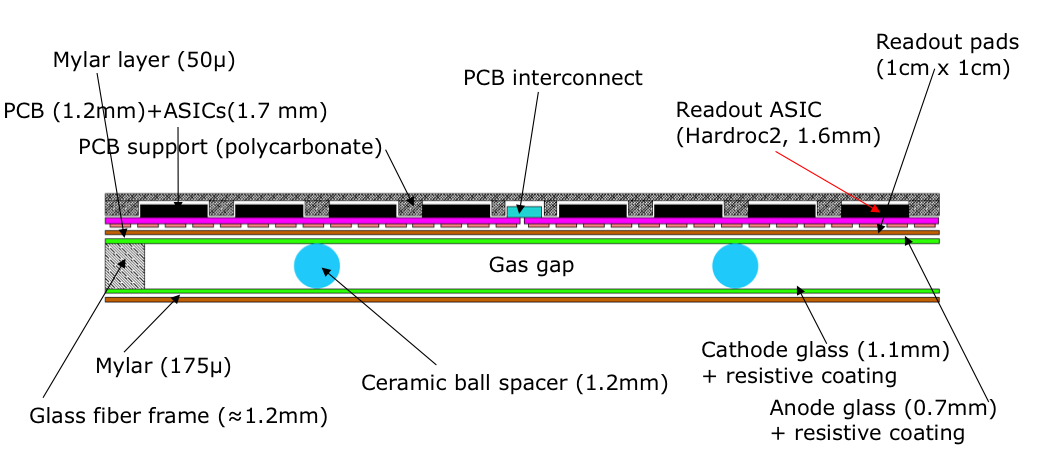
\includegraphics[width=.8\textwidth]{SDHCAL/figs/GRPC-K7.png}
    \caption{Schéma d'une GRPC.}
    \label{fig:grpc}
  \end{center}
\end{figure}
L'anode et la cathode ont des épaisseurs de 0.7 et 1.1 $mm$ respectivement. La peinture appliquée sur ces électrodes est une peinture bi-composant à base de graphite colloïdal. Les électrodes sont séparés par une couche de gaz de 1.2 $mm$ d'épaisseur. Cette épaisseur est garantit par des billes en céramique de 1.2 $mm$ de diamètre collées sur les électrodes. Des carreau de cuivre capacitifs de 1 $cm^2$ (figure~\ref{fig:carreaux}) utilisés pour collecter la charge sont directement imprimer de l'autre coté du circuit de lecture. Chaque GRPC contient 9216 carreaux de cuivre, ce qui conduit à plus de de 440000 canaux de lecture pour le prototype.
\begin{figure}[!h]
  \begin{center}
    \includegraphics[width=.8\textwidth]{SDHCAL/figs/PADs.png}
    \caption{Les carreaux de cuivres capacitifs de 1 $cm^2$ imprimés de l'autre coté du circuit de lecture d'une petite chambre utilisée pendant le développement du détecteur.}
    \label{fig:carreaux}
  \end{center}
\end{figure}
Une feuille de Mylar de 50 $\mu m$ est déposée entre l'anode et les carreaux de cuivre pour isoler ces derniers. Le circuit de imprimé lecture PCB (Printed Circuit Board) est composé de 6 ASUs (Active Sensor Unit) soudés entre eux. Sur chaque ASU, 24 ASICs (Application Specifique Integrated Circuit) HARDROC2~\cite{omega} sont déposés (figure~\ref{fig:layer}(b)). 
\begin{figure}[!h]
  \begin{center}
    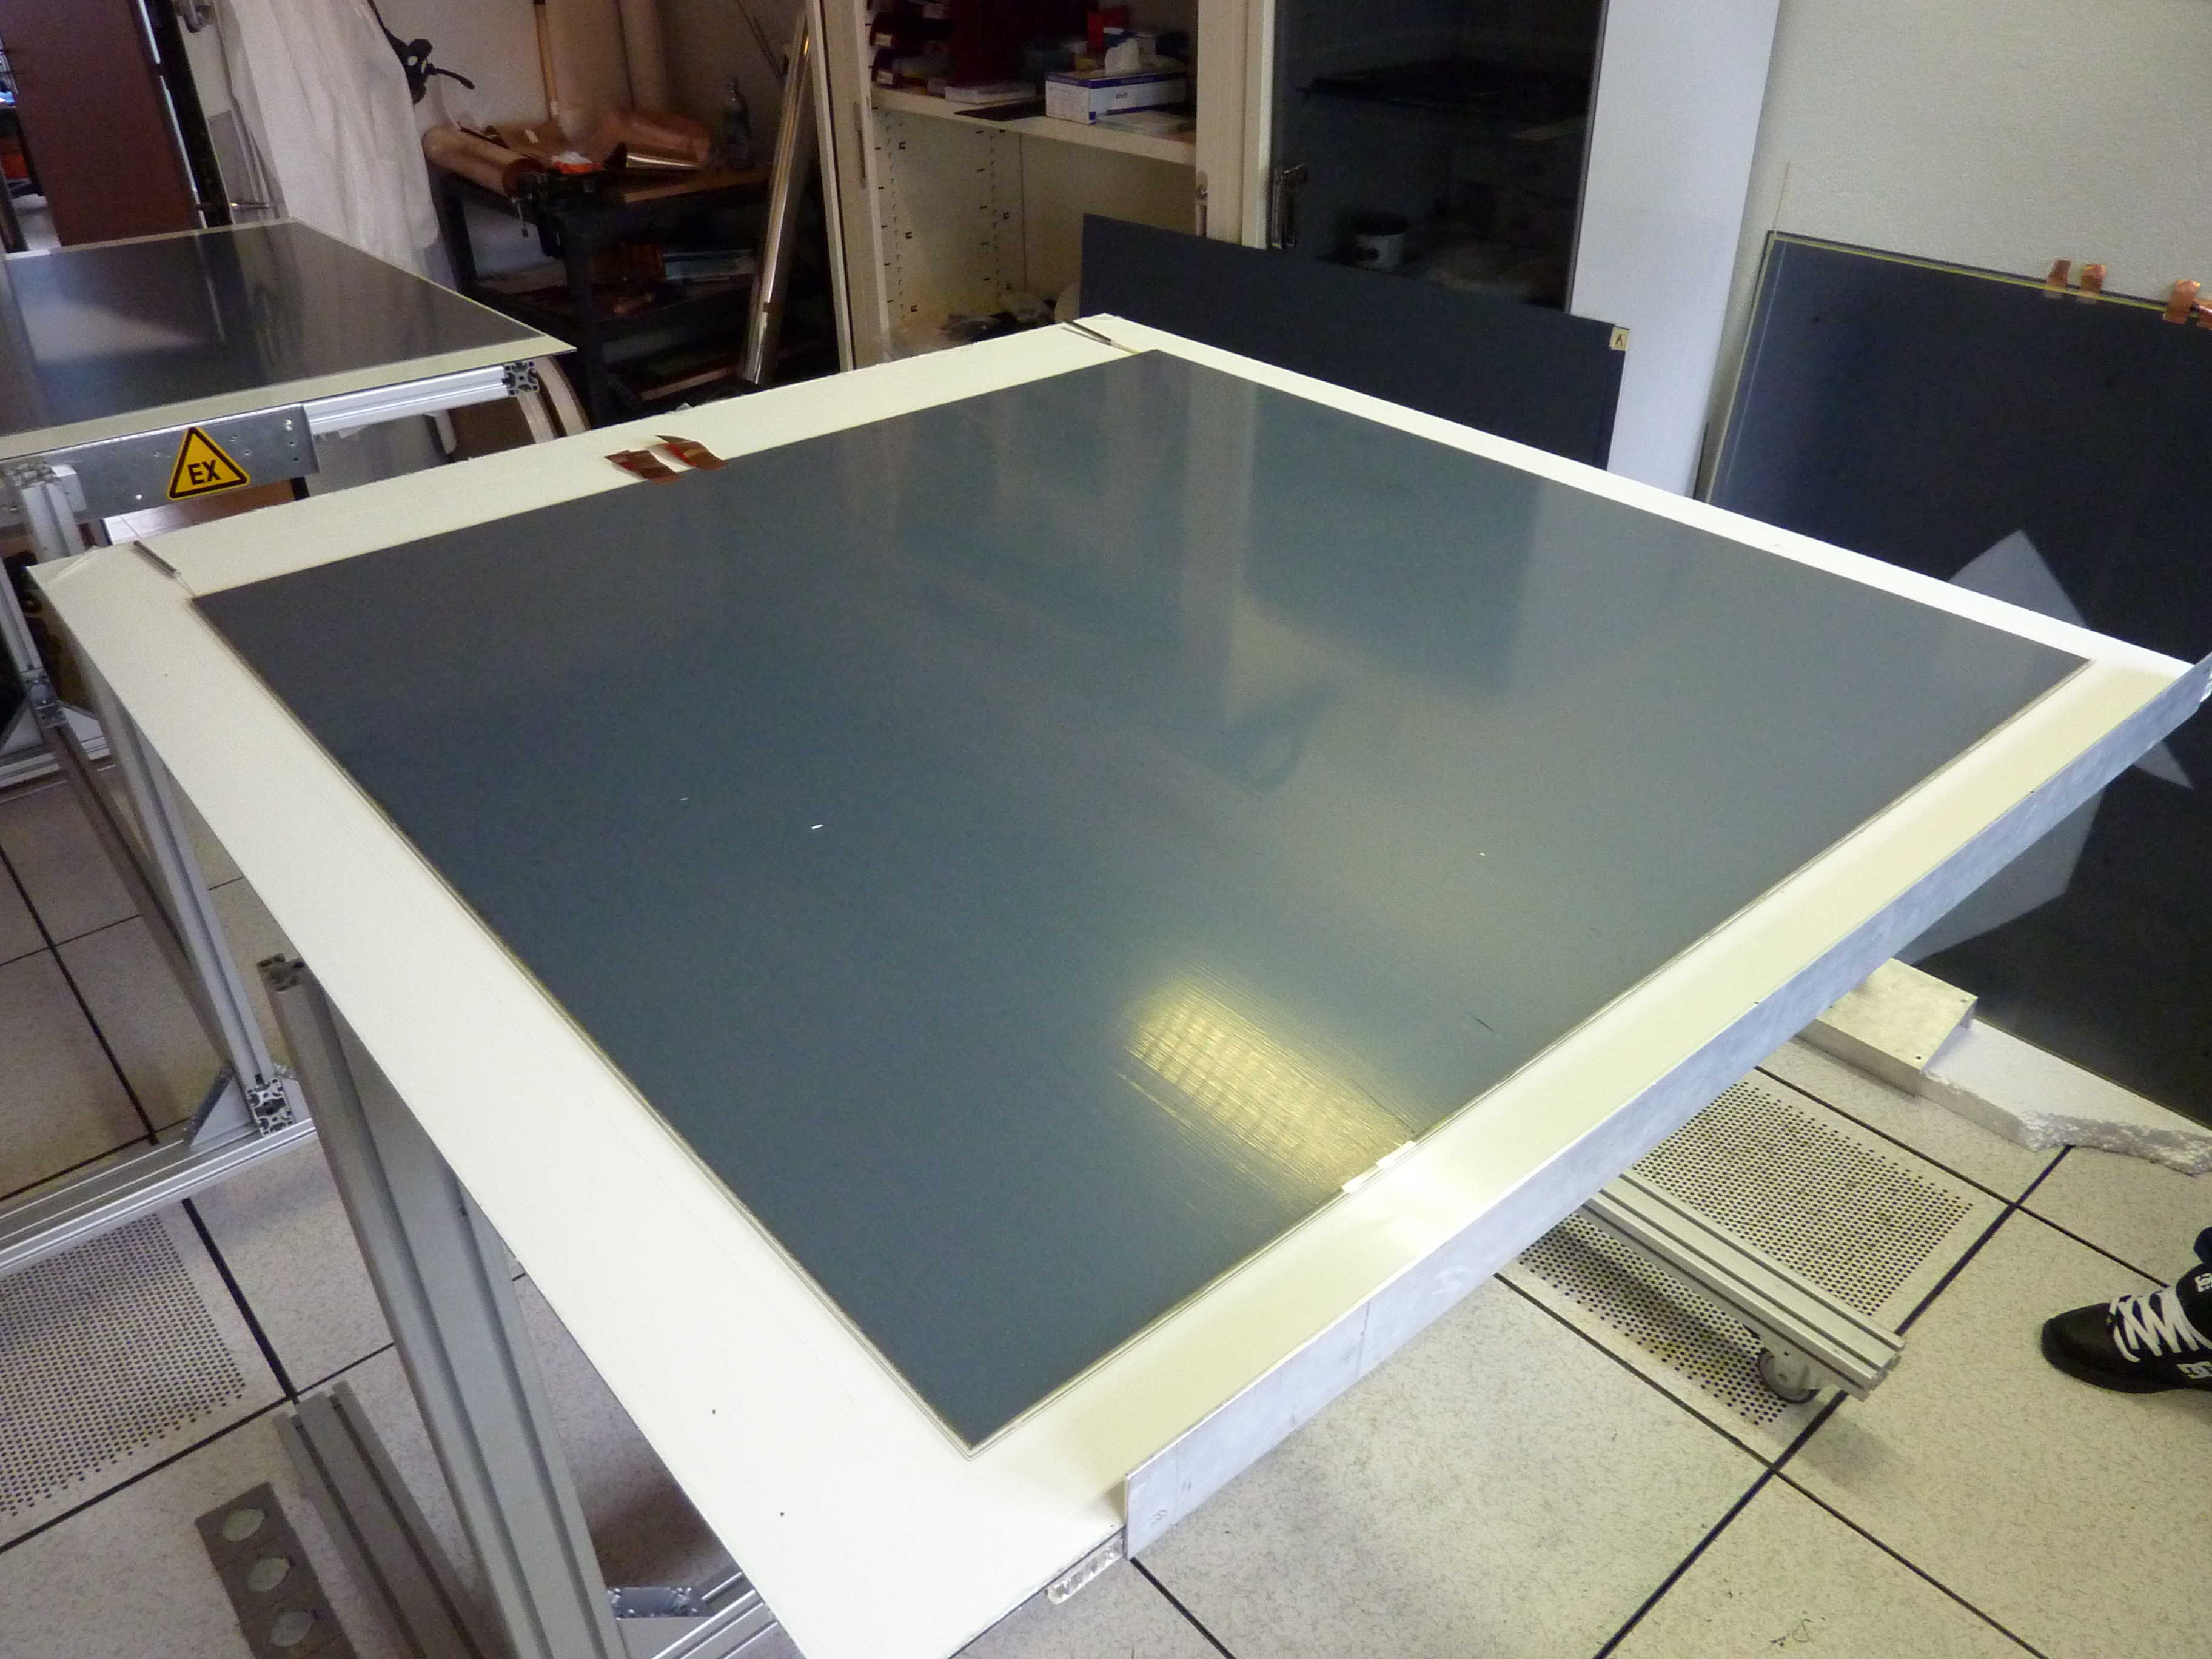
\includegraphics[width=.47\textwidth]{SDHCAL/figs/aLayer.jpg}
    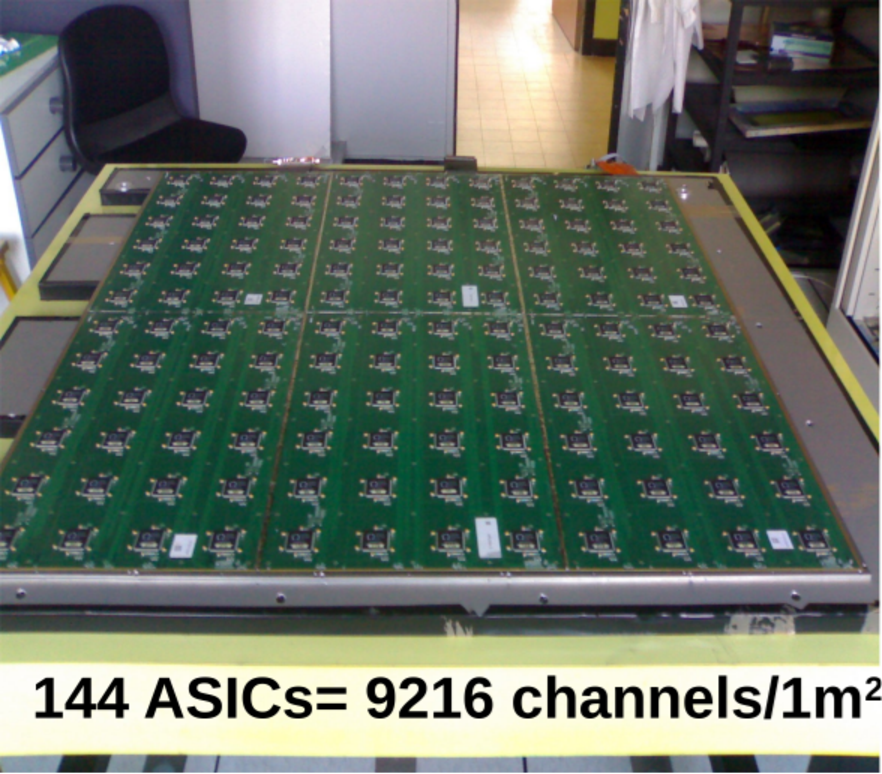
\includegraphics[width=.4\textwidth]{SDHCAL/figs/layer_electronic2.pdf}
    \caption{Photographie d'une GRPC sans son électronique ni sa cassette (à gauche) et d'un circuit imprimé de lecture (à droite) sur lequel on distingue les 144 ASICs.}
    \label{fig:layer}
  \end{center}
\end{figure}
Chacun de ces ASICs sont reliés à 64 carreaux de cuivre. Ces ASICs collectent les signaux des carreaux de cuivre, puis ces signaux sont amplifiés et trois discriminateur en font l'analyse pour déterminer le seuil des signaux. Trois cartes interfaces détecteur DIF (Detector Interface) par GRPC font le lien entre les ASICs et les ordinateurs d'acquisition. Les paramètres de l'acquisition (valeurs des seuils, des gains...) sont envoyés aux ASICs via ces DIFs. La figure~\ref{fig:DIF} montre une photographie du haut d'une GRPC avec ses trois DIFs connectées au PCB.
\begin{figure}[!h]
  \begin{center}
    \includegraphics[width=.4\textwidth,angle=90]{SDHCAL/figs/DIFCassette.jpg}
    \caption{Photographie du haut d'une GRPC avec ses trois DIF connectées au PCB.}
    \label{fig:DIF}
  \end{center}
\end{figure}

\subsection{Alimentation pulsée}
Le prototype du SDHCAL possède déjà plus de 440000 canaux de lecture. Le calorimètre hadronique finale d'une expérience telle que l'ILD comportera plus de 50 millions de cellules de 1 $cm^2$. L'énergie dissipée avec des cellules de lecture classique sera telle que l'utilisation de système de refroidissement des calorimètre deviendrait indispensable. Or ces systèmes auraient un budget matière non négligeable, ce qui dégraderait la résolution en énergie des jets. De plus pour utiliser des techniques de suivi des particules dans tous les sous détecteurs, il faut minimiser les zones non instrumentées. La volonté de construire des calorimètres ultra-granulaires a obligé les équipes chargées du développement de l'accélérateur à prendre en compte ces contraintes pour le future ILC. Ainsi, le système d'accélérateur à l'ILC ne délivrera du faisceau que pendant 0.95 $ms$ toute le 200 $ms$ \cite{acceleratorTDR}. La figure~\ref{fig:ILCCycle} montre un schéma de la structure temporelle du faisceau de l'ILC.
\begin{figure}[!h]
  \begin{center}
    \includegraphics[width=.8\textwidth]{SDHCAL/figs/PPCycle.pdf}
    \caption{Schéma de la structure temporelle du faisceau de l'ILC.}
    \label{fig:ILCCycle}
  \end{center}
\end{figure}
Cette structure temporelle permettra de lire les données du détecteur lorsqu'il n'y a pas de faisceau. De plus, cela permet d'utiliser une alimentation pulsée pour les sous détecteurs. Certains composants des détecteurs ne seront allumés que pendant les collisions entre particules ($\Delta_t=0.95~ms$). Cela entraînera une forte réduction de dissipation thermique et aussi une diminution non négligeable de la consommation des détecteurs. Le prototype du SDHCAL a été le premier détecteur utilisant une alimentation pulsée. Lors des test en faisceau au SPS en 2012, du faisceau était délivré par la machine pendant 9 $s$ toutes les 45 $s$. Ainsi, les composants analogiques des ASICs qui sont les composants ayant la plus forte consommation d'énergie, étaient éteints pendant les 34 $s$ sans faisceau. Les caractéristiques du SPS sont loin des futures caractéristiques du faisceau de l'ILC, et pour collecter des données dans de bonnes conditions un système de refroidissement du détecteur a été utilisé. Il est fait de plaques de cuivre collée des deux cotés du prototype dans lequel circule de l'eau refroidit à 10$\degres C$.

\subsection{Description d'un cycle d'acquisition}
Au début d'une phase d'acquisition, l'horloge interne des ASICs est remise à zéros. Les ASICs et les DIFs sont synchronisés à l'aide de DCCs (Data Concentrator Card) et d'une SDDC (Synchronous Data Concentrator Card). Le temps dans les ASICs et dans les DIFs est échantillonné par pas de 200 $ns$. Pendant une phase d'acquisition, lorsqu'un ou plusieurs des 64 canaux d'un ASIC passe le premier seuil, un événement est stockée dans la mémoire interne de l'ASIC. Chaque HARDROC peut enregistrer jusqu'à 127 événements de ce type. Lorsque la mémoire d'un des ASICs du détecteur est plein, un signal RAMfull est envoyé à tout le détecteur, l'acquisition est stoppée et les mémoires internes de tous les ASICs sont lus par les DIFs puis envoyés aux ordinateurs d’acquisition. Un événement RAMfull (la construction des événements physiques sera discuté dans la section~\ref{sec.trivent} de ce chapitre) est alors stocké sur disque. Les informations contenus dans ces événements sont les suivantes: 
\begin{enumerate}[1-]
\item le numéro de l'événement RAMfull
\item le temps absolue au moment du signal RAMfull (par pas de 200 $n$s) depuis le début de la prise de donnée
\item pour chaque coups:
  \begin{enumerate}[-]
    \item une clef unique permet de retrouver la position du carreau de cuivre. Dans cette clef on retrouve le numéros de la DIF (de 0 à 255), le numéro de l'ASIC (de 0 à 47) et enfin le numéro de canal (de 0 à 63).
    \item le temps (par pas de 200 $n$s) relatif au début du cycle d'acquisition
    \item le seuil déclenché par le signal induit sur le carreau de cuivre
  \end{enumerate}
\end{enumerate}
Après cette phase de lecture, un nouveau cycle d'acquisition démarre automatiquement. Ce mode d'acquisition a la particularité de ne pas utiliser de système de déclenchement externe ({\it{trigger}}). Les données collectées en test faisceau, contiendront donc des événements venant de particules du faisceau, des particules cosmiques et le bruit des détecteurs. Ce bruit est un paramètre important à contrôler. En effet si des canaux électroniques sont trop bruyant, ils seraient responsables de signaux RAMfull déclenchés immédiatement après le début du cycle et empêcheraient donc l'enregistrement de données. Ce mode de lecture sans déclenchement externe, rend obligatoire une procédure de reconstruction des événements dits physique que nous détaillerons dans la section~\ref{sec.trivent}.
\
\subsection{Le réglage des seuils}
\label{sec.sdhcal_thr}
Pour régler les trois seuils des GRPCs, un convertisseur digital-analogique (DAC), encodé sur 10 bits (de 0 à 1023), est utilisé pour chaque seuil. Les facteurs de conversion donnant le valeur du seuil sur la charge induite à partir de la valeur de DAC sont nécessaires pour la simulation. Un dispositif permet de d'injecter une charge donnée sur les 64 canaux des ASICs. Ce dispositif permet d'effectuer un scan sur la charge injectée. Pour chaque valeur de charge injectée, la valeur du seuil de basculement qui correspond à la valeur de DAC pour laquelle l'efficacité de détection est égale à 50\%, est mesurée \cite{kieffer}. Les courbes de ces valeurs en fonction de la charge injectée sont construites pour chaque canal des ASICs, pour chaque seuil. La figure~\ref{dac-vs-inj} montre un exemple de ces courbes pour les 64 canaux d'un ASIC, pour le premier seuils. 
\begin{figure}[!ht]
  \centering
  \includegraphics[width=.7\textwidth]{SDHCAL/figs/Dac0Lin.pdf}
  \caption{Seuil de basculement pour le premier seuil ($DAC_0$) en fonction de la charge injectée pour les 64 canaux d'un ASIC. La valeur du piédestal a été précédemment soustraite.}
  \label{dac-vs-inj}
\end{figure}
La valeur du piédestal a été précédemment soustraite pour la construction de ces courbes. La méthode pour extraire les valeurs des piédestaux pour chaque seuil est décrite dans \cite{kieffer}. Les courbes de la figure~\ref{dac-vs-inj} sont ajustées avec une droite. Finalement l'équation suivante permet d'obtenir la valeur du seuil en fonction de la valeur de DAC pour chaque seuil:
\begin{equation}
  seuil_i = \frac{DAC_i-p_i}{\lambda_i} [pC]
  \label{eq.dacConversion}
\end{equation}
où les coefficients $\lambda_i$ sont les valeurs moyennes des coefficients directeurs des droites obtenus après les ajustements linéaires et $p_i$ les valeurs des piédestaux.
Le tableau~\ref{tab.lambdas} présente les valeurs des facteurs de conversion et des piédestaux pour chaque seuil.
\begin{table}[!ht]
  \begin{center}
    \begin{tabular}{c|c|c}
      Seuil & $\lambda~[pC^{-1}]$ & Piédestal\\
      \hline
      1 & 700.0 & 90\\
      2 & 80.0 & 98\\
      3 & 16.3 & 98
    \end{tabular}
  \end{center}  
  \caption{Facteur de conversion et valeur des piédestaux pour chaque seuil.}
  \label{tab.lambdas}
\end{table}
Cependant, il n'était pas possible de réaliser les mesures des piédestaux et des facteurs de conversion avec les détecteurs complets. Les valeurs des piédestaux et des facteurs de conversion sont probablement légèrement différentes de celle obtenues (tableau~\ref{tab.lambdas}).

\subsection{Le fonctionnement d'une GRPC}
Le mode de fonctionnement des GRPCs dans le SDHCAL est le mode avalanche. Le mélange gazeux et la haute tension appliquée ont été choisi pour avoir une très bonne efficacité de détection et pour avoir une fréquence de détection raisonnable. 
\subsubsection{Le mélange de gaz}
Le mélange de gaz choisis est le suivant: $96\%$ de $TFE$, $5\%$ de $CO_2$ et $2\%$ de $SF_6$. Le $TFE$ a été choisi pour son potentiel d'ionisation (10.7 $eV$). Ce gaz est celui qui fournit les électrons de l'avalanche. Pendant le développement de l'avalanche, certaines molécules sont excitées. Leur désexcitation libère des photons. Ceux-ci risquent de ioniser d'autres molécules notamment grâce à l'effet photo-électrique et donc de déclencher des avalanches. Le $CO_2$ est utilisé pour limiter cet effet. Le $SF_6$ est gaz très électronégatif et permet d'absorber des électrons. Son effet sera de limiter la taille latérale de l'avalanche et aussi de réduire le bruit thermique.

\subsubsection{Réglage de la haute tension}
Pour régler les haute tension, l'efficacité en fonction de cette tension est étudiées. La figure~\ref{fig:plateau} monter l'efficacité de deux chambres du prototype en fonction de la tension. Sur ces courbes, on distingue deux zones. L'efficacité augmente presque linéairement avec la tension jusque 6.6 $kV$. Après 6.8 $kV$ on observe un plateau d'efficacité. 
\begin{figure}[!h]
  \begin{center}
    \includegraphics[width=.49\textwidth]{SDHCAL/figs/plateau12.png}
    \includegraphics[width=.49\textwidth]{SDHCAL/figs/plateau33.png}
    \caption{Courbes d'efficacité de deux GRPCs en fonction de la haute tension appliquée. Le plateau d'efficacité est atteint autour de 6.8 $kV$.}
    \label{fig:plateau}
  \end{center}
\end{figure}
La tension choisi doit ce situer sur le plateau. Ainsi, des variations des conditions extérieures (température, pression) n'auront que peu d'impact sur les gains des détecteurs. Pour les tests en faisceau de 2012, la haute tension appliquée sur les détecteurs était de 6.9 $kV$. Lors des tests de 2015, nous avons refait les courbes d'efficacité en fonction de la tension et nous avons réglé les tensions pour que tous les détecteurs soient au même endroit sur le plateau. Ces tensions variaient de 6.8 à 7.2 $kV$. De plus, lors de ces tests, les tensions étaient corrigées en fonction de la température extérieure et de la pression atmosphérique. 

\subsubsection{Seuils utilisés}
Les seuils ont été optimisé avec la simulation pour optimiser la résolution en énergie. Ils ont été fixés à 114 $fC$, 5 $pC$ et 15 $pC$. Cependant, ces réglages ont été effectuer avec une simulation peu réaliste et des études actuellement en cours pour ré-optimiser ces valeurs.

\subsection{Correction des gains}
\label{sec.gainCorrect}
Tous les canaux des ASICs possèdent un préamplificateur de charge. Ils sont utilisés pour augmenter ou diminuer le signal d'un canal avant l'entrée du signal dans les discriminateurs multipliant le signal par un gain allant de 0 à 2. Lors des tests en faisceau de 2012, tous les gains du prototype étaient régler à 1. Lors des tests en faisceau de 2015, nous avons mis en œuvre une méthode de correction de gains pour réduire le bruit dans le détecteur et aussi pour améliorer ses performances. Cette méthode est basée sur une analyse du bruit dans le prototype. Nous avons pris des données sans faisceau. Pour ne pas biaisé l'analyse, les événements physique (cf. section~\ref{sec.trivent}) sont rejetés. En effet, même sans faisceau il reste les particules cosmiques dans les échantillons de données. De plus, les bruits cohérents dus à des problèmes de masse sont aussi rejetés en demandant un nombre de coups inférieur à 50 dans chaque coup d'horloge de 200 $ns$. Il suffit alors de compter le nombre de coups enregistrés dans chaque canal pendant la prise de données. La figure~\ref{fig:noise_and_gain}(a) montre la distribution du nombre de coups de bruits de chaque canal lors d'une prise de donnée.
\begin{figure}[!ht]
  \subfigure[]{\includegraphics[width=.5\textwidth]{SDHCAL/figs/noise.pdf}}
  \subfigure[]{\includegraphics[width=.5\textwidth]{SDHCAL/figs/gain.pdf}}
  \caption{Distribution du nombre de coups de bruits pour chaque canal lors d'une prise de donnée (a). Gain calculée à partir de la distribution de Fermi-Dirac (b).\label{fig:noise_and_gain}}
\end{figure}
Les valeurs des nouveaux gains sont calculés pour chaque canal à l'aide de la fonction suivante:
\begin{equation}
  g_i=\frac{1}{1+e^{\frac{N_i-\tilde{N}}{\sigma_N}}}
\end{equation}
où $N_i$ correspond au nombre de coups de bruits dans le canal $i$, $\tilde N$ et $\sigma_N$ sont la valeur médiane et l'écart type de la distribution du bruits (figure~\ref{fig:noise_and_gain}(a)). La figure~\ref{fig:noise_and_gain}(b) montre la distribution des nouveaux gains. Cette distribution est alors normalisée pour avoir un gain moyen égale à 1: ces gains sont divisés par la valeur moyenne de la distribution des nouveaux gains (figure~\ref{fig:noise_and_gain}(b)). Ces nouveaux gains, permettent de masquer les canaux les plus bruyant et ainsi de prendre de données dans de meilleurs conditions. 
\begin{figure}[!ht]
  \subfigure[]{\includegraphics[width=.5\textwidth]{SDHCAL/figs/gainMap31.pdf}}
  \subfigure[]{\includegraphics[width=.5\textwidth]{SDHCAL/figs/noiseRate.pdf}}
  \caption{Carte des gains de la chambre 31 du prototype SDHCAL (a). Distribution du taux de bruits dans chaque canal avant (en noire) et après (en rouge) les corrections de gain (b).\label{fig:map_and_rate}}
\end{figure}
La figure~\ref{fig:map_and_rate}(a) montre un exemple de carte de gains pour une chambre du prototype. Les zones en bleu correspondent aux zones les plus bruyantes et sont presque masquées après la correction. Les zones blanches sont soit des zones non bruyantes, soit des zones déjà masqués. Le gains maximales est appliqué pour ces canaux. La figure~\ref{fig:map_and_rate}(a) montre la distribution du taux de bruits pour chaque canal avant et après les correction de gains. Après les correction de gains, le nombre de canal ayant un taux de bruits supérieur à 100 $Hz$ diminue sensiblement. Ceci a pour effet d'améliorer nos conditions de prise de données. En effet, le temps d'acquisition qui correspond au temps entre le début d'un cycle d'acquisition et le signal RAMfull augmente sensiblement après les corrections de gains (43 $ms$ après corrections contre 22 $ms$ avant). Cela nous permet d'obtenir la statistique d’événements intéressante pour l'analyse plus rapidement.

Les résultats obtenus avec les corrections de gains seront présentés et discutés dans la  section~\ref{sec.gainCorrectRes} de ce chapitre. Les autres résultats sont obtenus sans correction de gains.

%%%%%%%%%%%%%%%%%%%%%%%%%%%%%%%%%%%%%%%%%%%%%%%

\section{Reconstruction de l'énergie dans le SDHCAL}
Nous avons décrit le prototype du SDHCAL et particulièrement sec GRPCs qui composent sa partie active. Nous allons maintenant développer les différentes étapes de la reconstruction de l'énergie des hadrons incidents.
\subsection{Reconstruction des événements}
\label{sec.trivent}
Nous avons déjà mentionner que le mode de lecture du prototype utilisé en test sur faisceau rend obligatoire une procédure de reconstruction des événements. Dans les données collectées, on trouve les événements physiques (muons du faisceau et cosmiques, gerbes hadroniques et électromagnétique) et du bruit. Pour séparer les événements physiques du bruits, nous utilisons une méthode de groupement temporelle des coups \cite{sdhcal-com}. Pour chaque événement RAMfull, les coups sont classés en fonction de leur temps d’occurrence. Rappelons que ce temps est échantillonné par pas de 200 $ns$ grâce à l'horloge interne des ASICs. La figure~\ref{fig:time_spectrum} montre un exemple de la distribution du temps des coups dans un événement RAMfull. 
\begin{figure}[!h]
  \begin{center}
    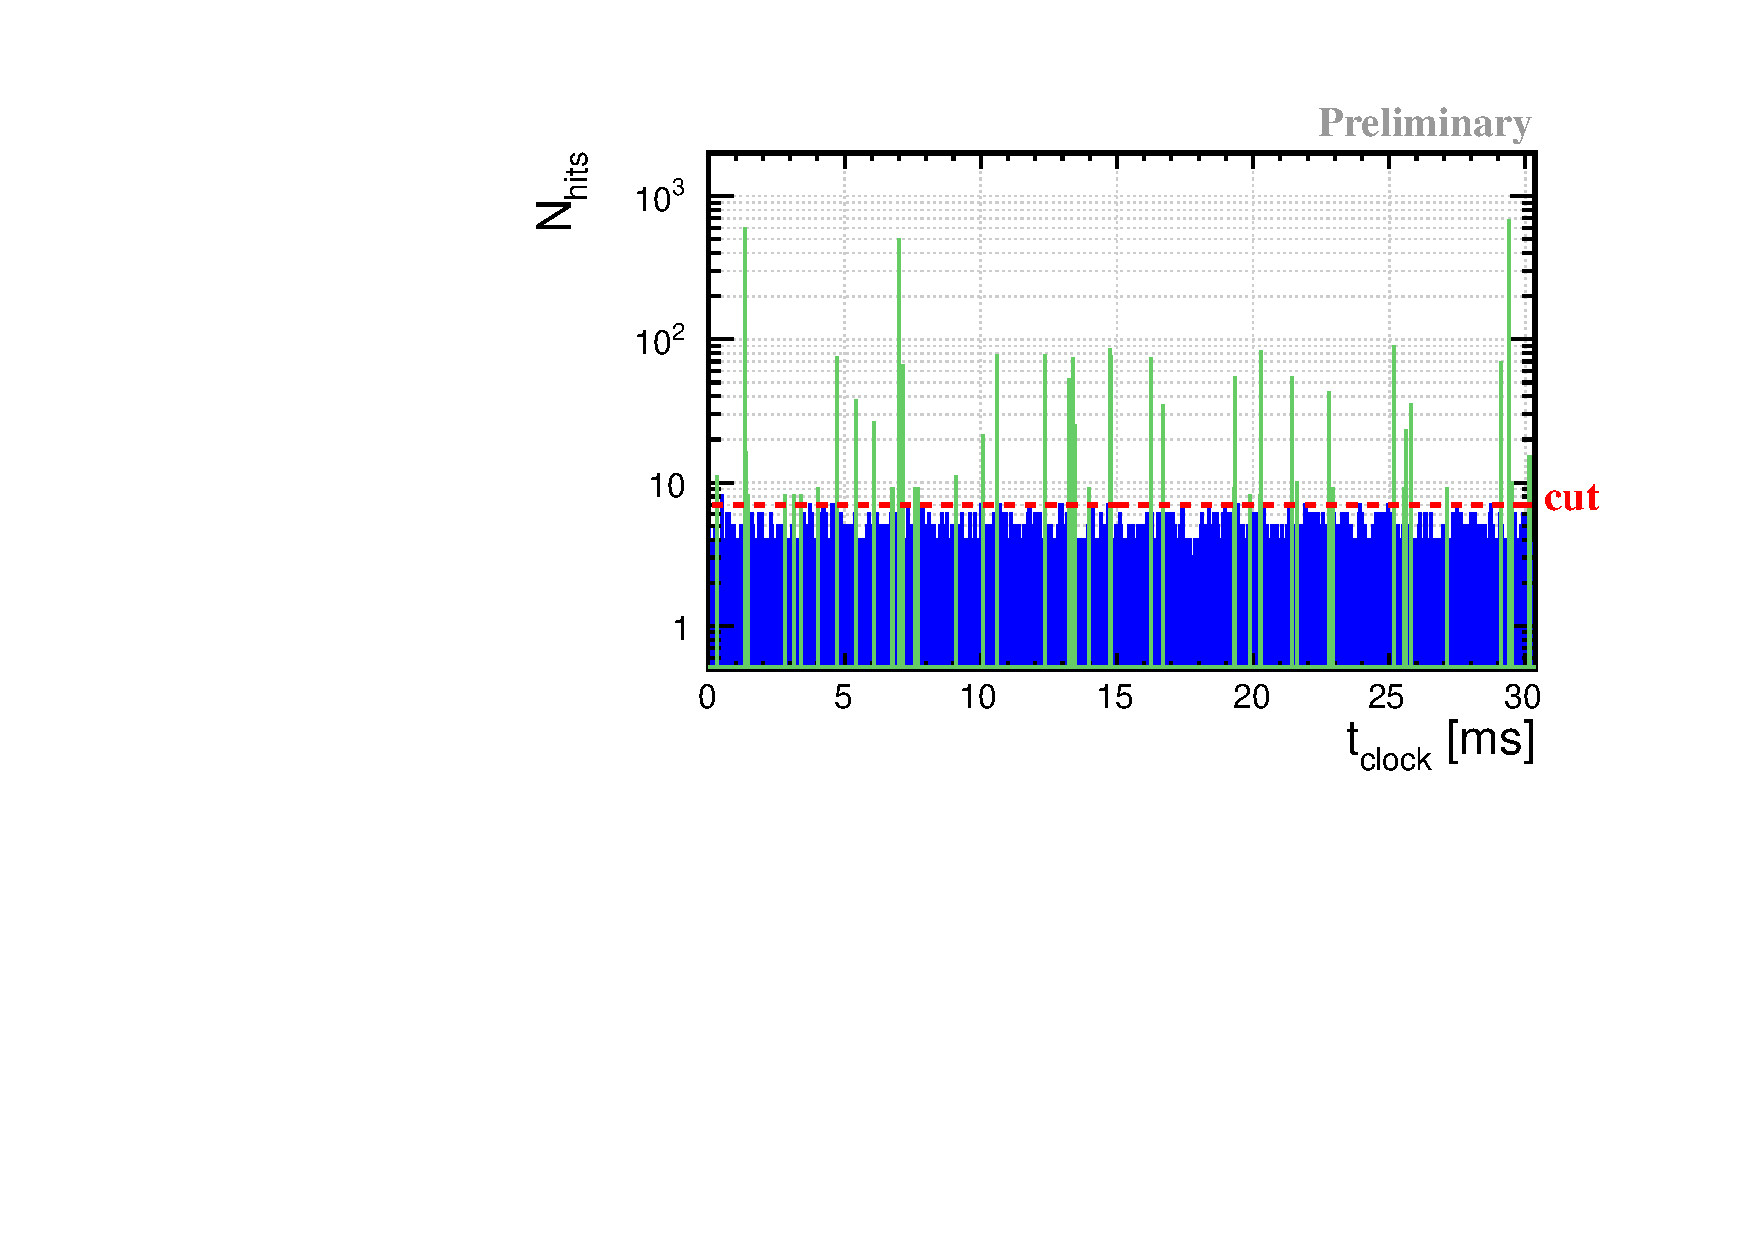
\includegraphics[width=.9\textwidth]{SDHCAL/figs/time_spectrum.pdf}
    \caption{Distribution du temps des coups dans un événement RAMfull. Les bins en vert correspondent au fenêtre en temps qui sont utilisés comme candidats d'événements physiques.}
    \label{fig:time_spectrum}
  \end{center}
\end{figure}
Lorsque dans un créneau d'horloge $t_0$ (1 créneau=200 $ns$), le nombre de coups est suffisant (>7 sur la figure~\ref{fig:time_spectrum}), un candidat d'événement physique est créé. Ce candidats est conservé seulement si il correspond à un maximum local ($\Delta_t=400~ns$) de la distribution de la figure~\ref{fig:time_spectrum}. Les coups dans les créneaux adjacents ($t=t_0\pm200~ns$) sont ajoutés au candidats. Cependant, il a été observé que certaines DIFs pouvaient légèrement se désynchroniser des autres. Un certain nombre de coup n'apparaissait pas dans l'événement et les gerbes hadroniques reconstruites semblaient "trouées". Ainsi, la fenêtre de temps pour construire les événements physiques a du être augmentée ($t=t_0\pm 2\times200~ns$). Un événement physique est finalement reconstruit si le nombre de plan de GRPCs avec au moins un coup est supérieur à un paramètre donné ($N_{plans}>=5$ par défaut). Le format des événements physiques est légèrement différent des événement RAMfull. Ils contiennent le temps du RAMfull, le temps relatif au début de leur cycle d'acquisition, les coordonnées des positions de touts les coups de l'événement physiques et leur seuil associé.

\subsection{Performance du SDHCAL}
\label{sec.muons}
Pour étudier les performances du prototype, l'efficacité et la multiplicité sont deux variables très importantes. L'efficacité correspond à la présence d'un signal détecté lors du passage d'une particule et la multiplicité correspond au nombre de canaux touchés lorsqu'une seule particule (MIP) traverse la couche de gaz. Ces deux variables correspondent aux propriétés intrinsèques des GRPCs. L'efficacité et la multiplicité sont étudiés pour de nombreuses applications. Les programmes de surveillance (monitoring) utilisé en test sur faisceau calculent ces variables ce qui permet rapidement de vérifier la qualité de la prise de données. Nous verrons dans le chapitre~\ref{chap.simulation} qu'une mesure précise de ces propriétés est indispensable pour la simulation du détecteur.
\subsubsection{Reconstruction des traces}
Pour étudier ces deux variables, qui représentent la réponse du détecteur au passage d'une seule particule, nous utilisons les événements muons. Ces événement sont reconstruits avec la procédure décrites dans la section~\ref{sec.trivent} de ce chapitre. Cependant, lors des test en faisceau nous n'avons pas pu utiliser de compteur Cerenkov pour identifier les particules. Il est donc nécessaire d'utiliser une procédure de sélection des événements muons et ainsi de rejeter les gerbes hadroniques et électromagnétiques présentes dans nos échantillons de données. Une analyse en composante principale PCA (Principal Component Analysis) permet aussi de sélectionner des candidats de traces. Une PCA consiste à diagonaliser la matrice des covariances. Cette matrice est une matrice $3\times3$ et ses éléments $M_{i,j}$ sont calculés avec l'équation suivante:
\begin{equation}
  M_{i,j}=\sum_{k=0}^{N_{coups}}{(x_{i,k}-\bar{x_j})(x_{j,k}-\bar{x_i})}
\end{equation}
où les $x_{i,k}$ sont les coordonnées positions des coups et les $\bar x_i$ sont les coordonnées du barycentre des coups de l'événement. Ces éléments sont ensuite normalisés avec la trace de cette matrice. Les valeurs propres $\lambda_i$ issues de la diagonalisation de la matrice sont classés par ordre décroissant. Le rapport $\frac{\sqrt{\lambda_2^2+\lambda_3^2}}{\lambda_1}$ est utilisé pour sélectionner les événements muons. La figure~\ref{fig:transverseRatio} montre ce rapport en fonction du nombre de coups. 
\begin{figure}[!h]
  \begin{center}
    \includegraphics[width=.7\textwidth]{SDHCAL/figs/transverseRatio.pdf}
    \caption{Rapport $\frac{\sqrt{\lambda_2^2+\lambda_3^2}}{\lambda_1}$ (Transverse Ratio) en fonction du nombre de coups ($N_{Hit}$) pour un échantillon de donnée à 30 $GeV$.}
    \label{fig:transverseRatio}
  \end{center}
\end{figure}
On peut facilement distinguer deux régions sur la figure~\ref{fig:transverseRatio}. La première région pour laquelle le nombre de coups est assez faible ($N_{Hit}<200$) correspond aux muons cosmiques et aux muons du faisceaux. La deuxième région ($N_{Hit}>200$) correspond au gerbes hadroniques. Une coupure sur la rapport $\frac{\sqrt{\lambda_2^2+\lambda_3^2}}{\lambda_1}$ à 0.05 permet de conserver une partie importante des muons tout en rejetant la plupart des gerbes hadroniques. Une deuxième procédure de sélection permet d'améliorer la qualité des traces sélectionnées et de rejeter les gerbes hadroniques restantes. Les étapes de cette sélection sont les suivantes:
\begin{enumerate}[-]
\item Les coups d'un même plan sont groupés lorsqu'ils se touchent. Les événements dont le nombre de groupes de coups est inférieur à une valeur donnée sont rejetés ($N_{groupes}<5$ par défaut).
\item La trajectoire de la particule est ajusté avec une régression linéaire dans les plans $xOz$ et $yOz$ (l'axe $Oz$ correspond à la direction du faisceau). Un $\chi^2$ de l'ajustement est calculé  avec l'équation suivante:
  \begin{equation}
    \chi^2=\frac{1}{N_{groupes}-1}\sum_{i=0}^{N_{groupes}}d_i^2
  \end{equation}
où les $d_i$ correspondent aux distances (en $mm$) entre le barycentre des groupes de coups et la droite définie par les coefficients obtenus lors des régressions linéaires. Les événements dont le $\chi^2$ est supérieur à 100 sont rejetés.
\end{enumerate}
\begin{figure}[!h]
  \begin{center}
    \includegraphics[width=.7\textwidth]{SDHCAL/figs/nhitMuon.pdf}
    \caption{Distribution du nombre de coups ($N_{Hit}$) après sélection des événements muons pour un échantillon de donnée à 30 GeV.}
    \label{fig:nhitMuon}
  \end{center}
\end{figure}
La figure~\ref{fig:nhitMuon} montre la distribution du nombre de coups ($N_{Hit}$) pour un échantillon de donnée à 30 GeV après les sélections des événements muons. On distingue deux pics sur cette figure. Le premier correspond aux muons cosmiques et le deuxième aux muons du faisceau.
\subsubsection{Efficacité et multiplicité}
Pour chaque muon reconstruit, l'efficacité est estimé pour chaque plan du détecteur susceptible d'être touché par la particule. Pour chacun de ces plans, l'impact de la trace est calculé avec une régression linéaire en utilisant la même méthode que précédemment. Les groupes de coups du plan étudié ne sont pas inclus dans la régression linéaire pour éviter un biais. Un plan est considéré comme efficace si un groupe de coups de trouvé à moins de 5 $cm$ de l'impact attendu. La multiplicité correspond alors au nombre de coups dans le groupe correspondant. 
\begin{figure}[!h]
  \begin{center}
    \includegraphics[width=.45\textwidth]{SDHCAL/figs/eff_2012.pdf}
    \includegraphics[width=.45\textwidth]{SDHCAL/figs/mul_2012.pdf}
    \caption{Efficacité (à gauche) et multiplicité (à droite) moyenne pour chaque chambre du SDHCAL.}
    \label{fig:eff_and_multi}
  \end{center}
\end{figure}
La figure~\ref{fig:eff_and_multi} montre les efficacités (a) et la multiplicité (b) pour chaque plan du prototype. L'efficacité moyenne du détecteur est de 96$\%$ et la multiplicité moyenne de 1.76. La dispersion autour de la multiplicité moyenne est élevée. Cette dispersion est probablement due à des différences de résistivité de la peinture appliquée sur les électrodes d'une chambre à l'autre.
\subsection{Sélection des gerbes hadroniques}
\label{sec.pi_selection}
Nous avons vu la procédure pour sélectionner les événements muons pour calculer l'efficacité et la multiplicité des GRPCs. Nous allons maintenant décrire la procédure pour sélectionner les gerbes hadroniques. Rappelons que les échantillons de données contiennent des muons (cosmiques et du faisceau), des gerbes hadroniques et électromagnétiques.
\subsubsection{Axe des événements}
L'axe des gerbes événements est une propriété qui sera utilisée à plusieurs reprises dans les paragraphes suivants. Pour construire cet axe, la méthode utilisée ressemble à la méthode décrite dans la section~\ref{sec.muons}. Un ajustement linéaire est réalisé en utilisant les coordonnées de tous les coups de l'événement. Cet axe est ensuite utilisé pour déterminer le point d'impact de la particule dans le prototype et l'angle entre la particule et l'axe $(Oz)$.
\subsubsection{Contamination par les protons}
Le faisceau de la ligne H6 du SPS est contaminé par des protons. Les protons produisent des gerbes hadroniques qui seront très difficilement différenciables de celles des pions. La collaboration ATLAS a mesuré la contamination de la ligne H6 \cite{Abat}. Le tableau suivant présente la fraction $f_p$ du nombre de protons sur le nombre totale de particules sur la ligne H6 pour 50 et 100 $GeV$:
\begin{table}[!ht]
  \begin{center}
    \begin{tabular}{c|c}
      Énergie & $f_p$\\
      \hline
      50 & $0.45\pm0.12$\\
      100 & $0.61\pm0.06$\\
    \end{tabular}
  \end{center}  
  \caption{Fraction du nombre de proton sur la ligne H6 du SPS.}
  \label{tab.fp}
\end{table}
Dans la suite, aucun traitement ne sera effectué pour identifier les gerbes hadroniques induites par les protons. Celles-ci seront traitées de la même façon que pour les pions. Cependant, la longueur d’interaction est légèrement plus faible pour les protons que pour les pions. La collaboration ATLAS a aussi mesuré le rapport des longueurs d’interactions des pions et des protons avec un calorimètre à échantillonnage utilisant des scintillateurs comme milieu actif et du fer en absorbeur. Le résultats de cette mesure est le suivant:
\begin{equation}
  \lambda_{pi}/\lambda_{p}=1.25\pm0.01_{stat}{}_{-0.01syst}^{+0.04}
\end{equation}
Cette mesure est en bon accord avec la valeur théorique de 1.22. Ainsi, les protons interagissent plus vite dans le fer. Ceci aura pour effet de limiter l'effet de fuites des gerbes hadroniques et donc d'augmenter le nombre de coups détecter. 
\subsubsection{Contamination par les muons}
Les coupures suivantes permettent de supprimer une importante fraction de la contamination des données par les muons.
\begin{enumerate}[-]
\item $\frac{N_{coups}}{N_{plans}}>3$, où $N_{plans}$ correspond au nombre de plan avec au moins 1 coup.
\item $\frac{\sqrt{\lambda_2^2+\lambda_3^2}}{\lambda_1}>0.01$, où $\frac{\sqrt{\lambda_2^2+\lambda_3^2}}{\lambda_1}$ correspond au rapport des valeurs propres après une analyse en composantes principales (cf. section~\ref{sec.muons}).
\item $\frac{N_{IP}}{N_{plans}}>0.1$, où $N_{IP}$ correspond au nombre de plans pour lesquels l'écart type de la position des coups est supérieur à 5 $cm$. Cette coupure permet de rejeter les muons radiatifs. 
\end{enumerate}
\begin{figure}[!h]
  \begin{center}
    \includegraphics[width=.8\textwidth]{SDHCAL/figs/muCut715747.pdf}
    \caption{Distribution du nombre de coups avant (en noir) et après (en bleu) l'application des coupures pour rejeter les événements muons à 30 GeV.}
    \label{fig:muCut}
  \end{center}
\end{figure}
La figure~\ref{fig:muCut} montre la distribution du nombre de coups pour un échantillon de données à 30 GeV, avant et après l'application des coupures pour rejeter les muons.
\subsubsection{Contamination par les gerbes électromagnétiques}
Pour supprimer les événements induits par des électrons, au moins une des trois coupures suivantes doit être vérifiée:
\begin{enumerate}[-]
\item $N_{Traces}>0$, où $N_{Traces}$ correspond au nombre de traces reconstruites en utilisant la technique de Transformée de Hough (voir section~\ref{sec.hough} du chapitre~\ref{chap.topo}). Si une trace reconstruite débute dans les trois premiers plans et que l'angle entre cette trace et l'axe $(Oz)$ est faible (<25$\degree$) alors elle définie la trace primaire. 
\item $P_{Start}\geq5$, où $P_{Start}$ correspond au premier plan d’interaction. Il est définit comme étant le premier plan avec un groupe avec plus de 4 coups. Ce plan doit se trouver après le dernier plan de la trace primaire. Le barycentre du groupe de coups correspondant doit être situé à moins de 10 $cm$ de l'impact attendue de la trace primaire. Si aucune trace primaire n'est reconstruite, alors le premier plan avec un groupe de plus de 4 coups proche de l'axe de la gerbe définit le premier plan d’interaction.
\item $N_{Plans}>30$
\end{enumerate}
\begin{figure}[!ht]
  \subfigure[]{\includegraphics[width=.3\textwidth]{SDHCAL/figs/ntrack_e-_50GeV.pdf}}
  \subfigure[]{\includegraphics[width=.3\textwidth]{SDHCAL/figs/zbegin_e-_50GeV.pdf}}
  \subfigure[]{\includegraphics[width=.3\textwidth]{SDHCAL/figs/nlayer_e-_50GeV.pdf}}
  \caption{Distribution du nombre de coups de bruits pour chaque canal lors d'une prise de donnée (a). Gain calculée à partir de la distribution de Fermi-Dirac (b).\label{fig:electron_control}}
\end{figure}
La figure~\ref{fig:electron_control} montre les distributions des trois variables utilisées pour rejeter les électrons. Ces distributions proviennent de simulation d'électron à 50 $GeV$. Pour chacune des variables, les rapports $\frac{N_{Events}|Var>cut}{N_{Events}}$ donnent la proportion d'événements non rejetés par les coupures définies ci-dessus. Ces rapports permettent d'affirmer que la proportion de gerbes électromagnétiques identifiée comme gerbes hadroniques sera faible. Cependant, la contamination du faisceau par les électrons n'était pas parfaitement maîtrisée malgré l'utilisation d'une fine couche d'absorbeur en plomb.
\subsubsection{Coupures supplémentaires}
La figure~\ref{fig:muCut} montre que les échantillons de données sont toujours contaminés, notamment dans la région de faible nombre de coups, malgré les coupures déjà appliquées. Quelques coupures supplémentaires sont nécessaire pour purifier les échantillons de données. 
\begin{enumerate}[-]
\item Les événements multiples sont filtrés en étudiant la dispersion des coups dans les 5 premiers plans. Ces événements sont issus la plupart du temps d’interactions de la particule incidente en amont du prototype (interactions avec les collimateurs, la couche de plomb, avec les détecteurs permettant le réglage du faisceau...). Si des coups sont séparés de plus de 5 $cm$ dans 4 des 5 premiers plans alors l'événement est considéré comme multiple. 
\item Les particules neutres sont filtrées en imposant la présence d'au moins 4 coups dans les 5 premiers plans.
\item L'angle entre la particule incidente et l'axe $(Oz)$ doit être inférieur à 25$\degree$. Cette coupure permet d'éliminer des événements où la particule incidente aurait légèrement interagi avant le prototype.
\end{enumerate}
\label{sec.shower_selection}
\begin{figure}[!h]
  \begin{center}
    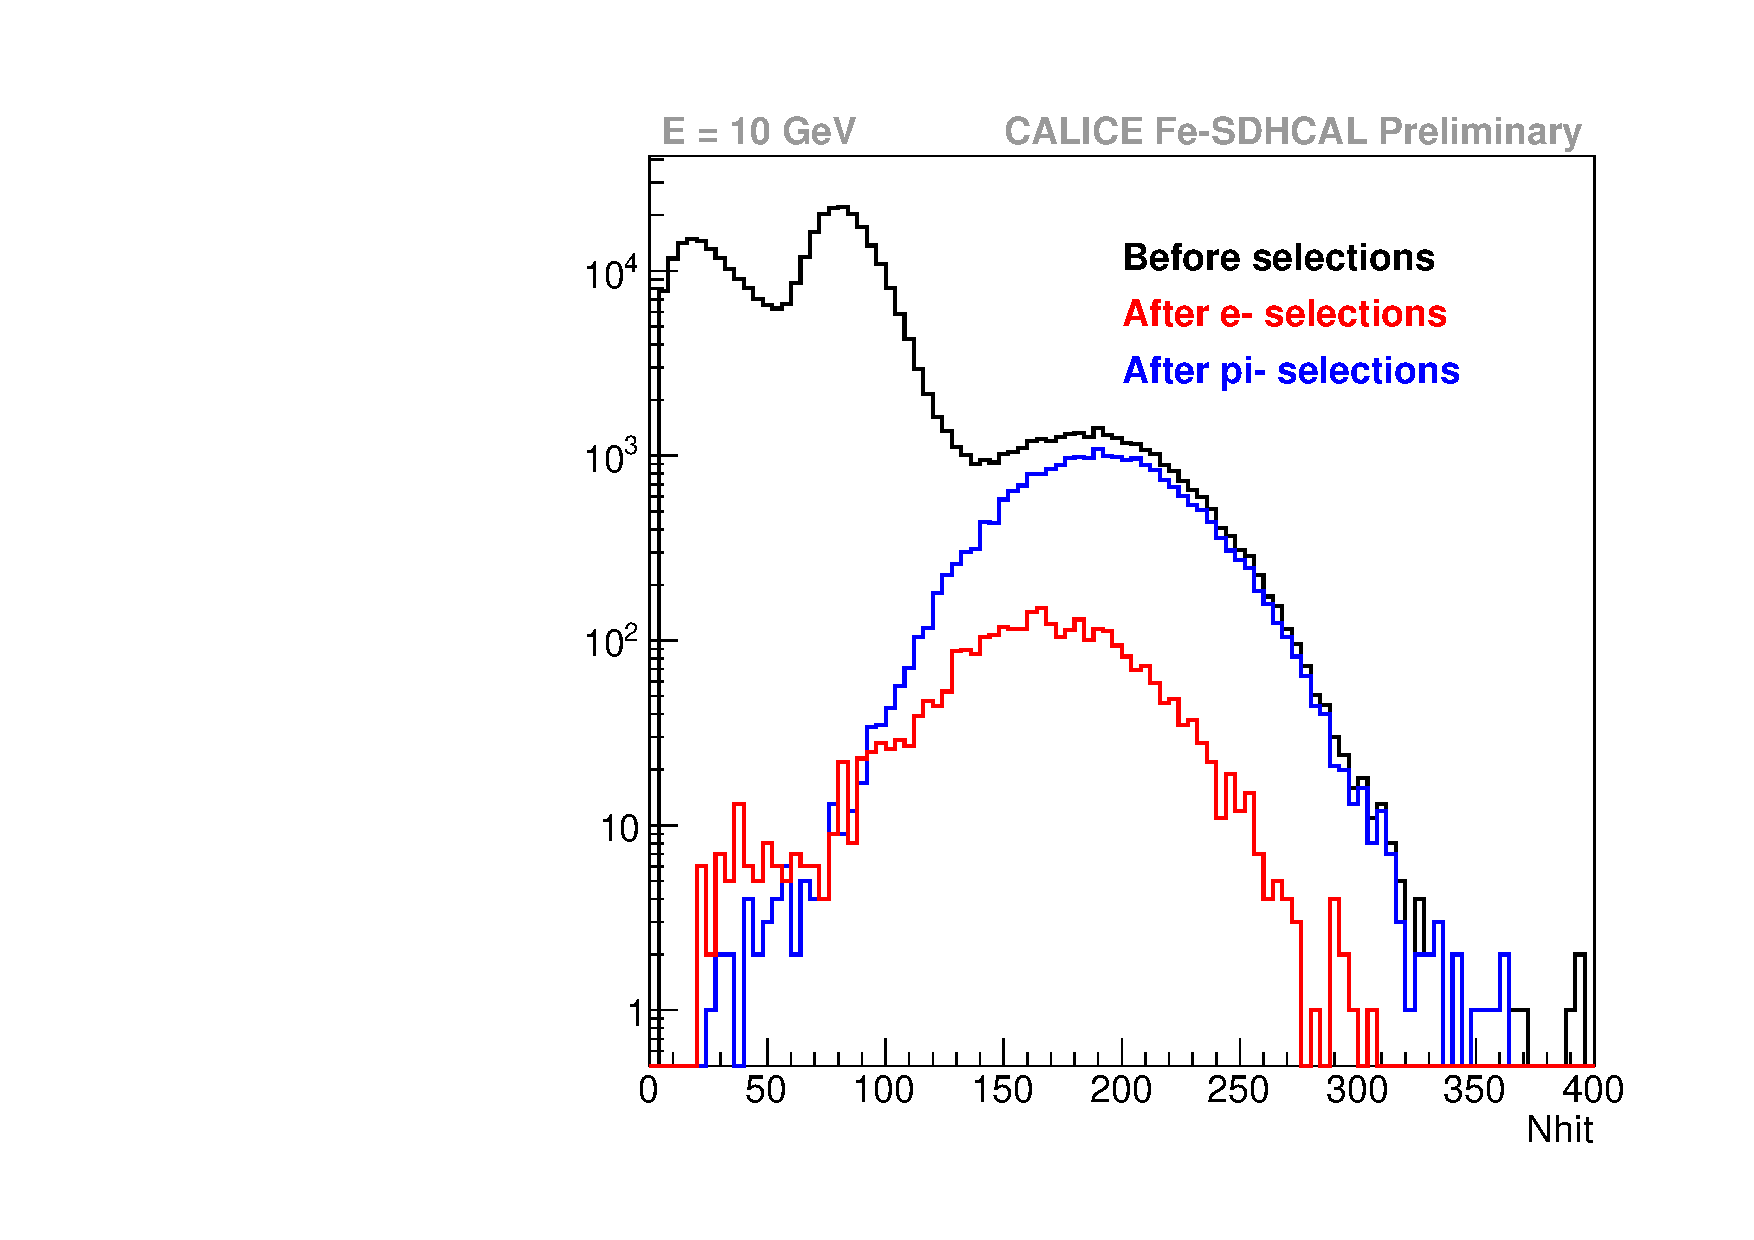
\includegraphics[width=.45\textwidth]{SDHCAL/figs/selection715693.pdf}
    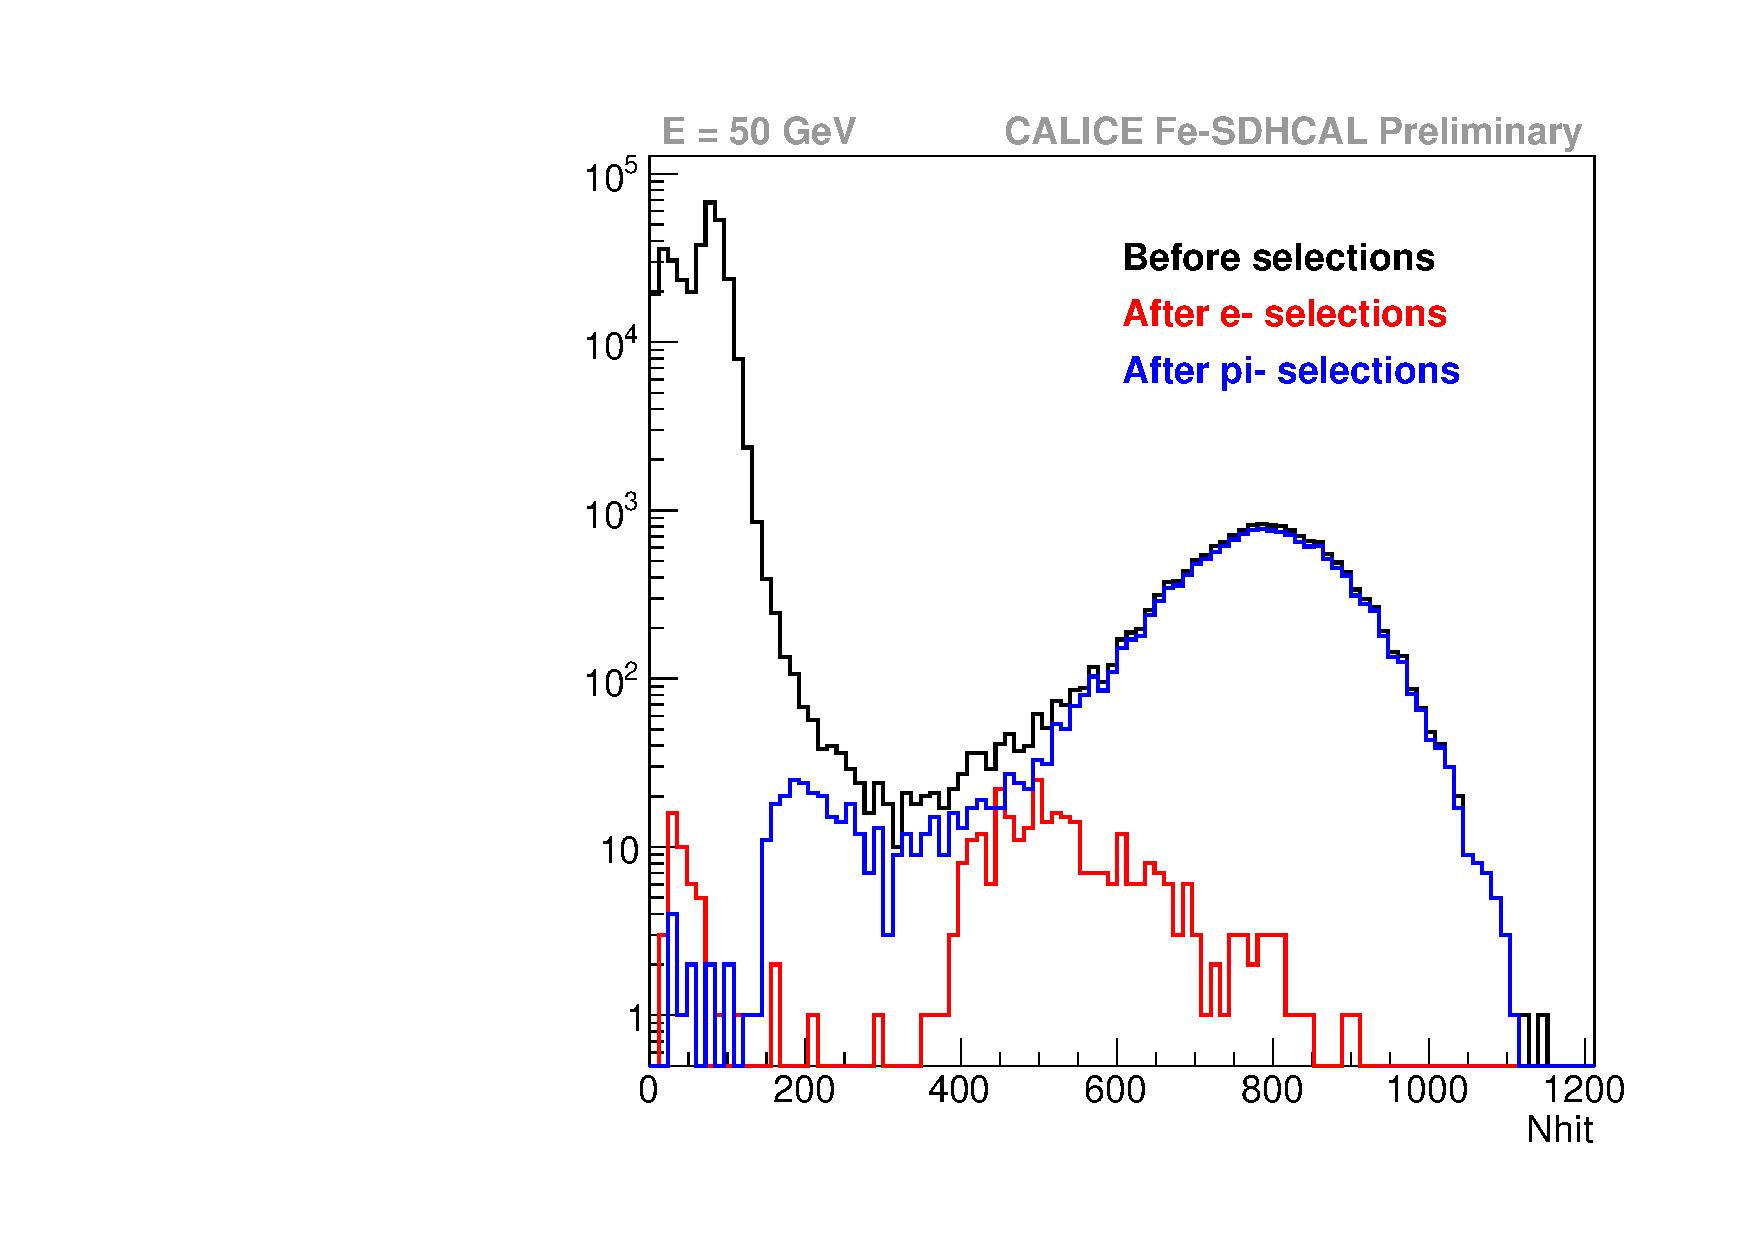
\includegraphics[width=.45\textwidth]{SDHCAL/figs/selection715751.pdf}
    \caption{Distribution du nombre de coups pour des échantillons de données à 10 (à gauche) et 50 (à droite) $GeV$ avant toutes les coupures (en noir) après les coupures de sélection des gerbes hadroniques (en bleu) et après les coupures de sélection des gerbes électromagnétiques (en rouge).}
    \label{fig:pion_selection}
  \end{center}
\end{figure}
La figure présente les distributions de nombre de coups pour des échantillons de données à 10 et 50 $GeV$ avant toutes les coupures (en noir) et après les coupures de sélection des gerbes hadroniques (en bleu). Les distributions après coupures de sélection des électrons sont aussi présentes. Nous détaillerons la procédure de sélection des électrons dans la section~\ref{sec.resultats} du chapitre~\ref{chap.simulation}. Les coupures que nous venons de détailler ont été accorder pour purifier au maximum les échantillons de données tout en essayant d'introduire un minimum de biais.
\begin{table}[!ht]
  \begin{center}
    \begin{tabular}{c|c}
      Energie & Efficacité \\
      \hline
      $5 ~GeV$ & $56.6\%$  \\
      $10~GeV$ & $84.4\%$ \\
      $15~GeV$ & $89.3\%$ \\
      $20~GeV$ & $91.2\%$ \\
      $25~GeV$ & $93.1\%$ \\
      $30~GeV$ & $93.6\%$ \\
      $40~GeV$ & $94.6\%$ \\
      $50~GeV$ & $94.6\%$ \\
      $60~GeV$ & $94.9\%$ \\
      $70~GeV$ & $94.4\%$ \\
      $80~GeV$ & $94.2\%$ \\
    \end{tabular}
  \end{center}  
  \caption{Efficacité de sélection des gerbes hadroniques en fonction de l'énergie de la particule incidente.}
  \label{tab.pi-selection}
\end{table}
Le tableau~\ref{tab.pi-selection} présente l'efficacité de sélection des gerbes hadroniques en fonction de l'énergie incidente. Cette efficacité est mesurée avec la simulation et correspond au rapport entre le nombre d'événements simulés et le nombre d'événements identifiés comme gerbes hadroniques. Ces efficacités sont satisfaisantes excepté à 5 $GeV$. Environ 20$\%$ des gerbes hadroniques simulées à 5 $GeV$ sont rejetées par les coupures muons, 20 $\%$ par les coupures électrons et environ 10$\%$ sont rejetées à cause de la coupure sur l'angle de la gerbe. Ceci est due au fait qu'à 5 $GeV$, la particule incidente subi le phénomène de diffusion multiple dans les couches d'absorbeurs. En comparaison, aucun événements de gerbe hadronique simulés à 80 $GeV$ n'est rejeté par cette coupure.
\subsection{Calibration en fonction du temps}
\label{sec.timeCalib}
Dans la section~\ref{sec.grpc} de ce chapitre, nous avons déjà expliqué que la résistivité des électrodes est un paramètre très important pour les RPC. La résistivité volumique du verre utilisé pour le SDHCAL est très élevée ($\rho=10^{12}~\Omega cm$). Cette résistivité élevée a pour conséquence de fortement dégrader l'efficacité de détection des GRPCs lorsque le flux de particules augmente. La figure~\ref{fig:eff_vs_rate} présente l'efficacité de détection de différentes GRPCs en fonction du taux de particules incidentes~\cite{haddad}. 
\begin{figure}[!h]
  \begin{center}
    \includegraphics[width=.6\textwidth]{SDHCAL/figs/EFFRate.pdf}
    \caption{Efficacité de détection en fonction du taux de particules incidentes.}
    \label{fig:eff_vs_rate}
  \end{center}
\end{figure}
L'efficacité de la chambre avec du verre standard (Float Glass, courbe orange) chute très rapidement lorsque le taux augmente. Les GRPCs construites avec du verre semi-conducteur, fabriqués à l'université de Tsinghua en Chine \cite{yi_wang}, ont une résistivité plus faible que les GRPCs du SDHCAL ($\rho=10^{10}~\Omega cm$). Cette résistivité leur permet de conserver une bonne efficacité malgré un fort taux de particules.
Cet effet est encore plus important avec les gerbes hadroniques et électromagnétiques où la densité de particules secondaires est très élevées.
\begin{figure}[!h]
  \begin{center}
    \includegraphics[width=.7\textwidth]{SDHCAL/figs/timeCalib70.pdf}
    \caption{Nombre moyen de coups pour des gerbes hadroniques de 70 $GeV$ en fonction du temps relatif au début d'un cycle du SPS.}
    \label{fig:time_correction}
  \end{center}
\end{figure}
La figure~\ref{fig:time_correction} montre le nombre moyen de coups pour des gerbes hadroniques de 70 $GeV$ en fonction du temps relatif au début d'un cycle du SPS en 2012. Pour construire cette figure, le temps relatif au début du cycle du SPS est reconstruit en imposant le début d'un nouveau cycle, lorsque plus de cinq secondes s'écoulent entre deux événements consécutifs. Le nombre de coup décroit sensiblement avec le temps. Cet effet augmente avec l'énergie du faisceau. En effet, à plus haute énergie, le nombre de particules secondaires augmente et donc le charge déposée sur les électrodes. Le temps pour neutraliser ces charges est donc légèrement plus long. Une procédure de calibration permet cependant de corriger cet effet. Les courbes de nombre de coups pour chaque seuil sont sont ajustées avec un polynôme d'ordre 2. Le nombre de coups pour chaque seuil, pour chaque événement, est corrigé avec la fonction suivante:
\begin{equation}
  N_{corr,i}=N_i-\sum_{j=0}^{2}p_{j,i}t^j
\end{equation}
où $i$ correspond au seuil, $N_{corr,i}$ est le nombre corrigé de coups pour le seuil $i$, les $p_{j,i}$ sont les coefficients de correction obtenus avec les ajustements et $t$ est le temps relatif au début du cycle du SPS.
\begin{figure}[!ht]
  \begin{center}
    \includegraphics[width=.7\textwidth]{SDHCAL/figs/calibnhit3_70.pdf}
    \caption{Distribution du nombre de coups pour le troisième seuil à 70 $GeV$ avant (en noire) et après (en rouge) les corrections temporelles.}
    \label{fig:nhit3_corrected}
  \end{center}
\end{figure}
La figure~\ref{fig:nhit3_corrected} montre les distributions du nombre de coups pour le troisième seuils à 70 $GeV$ avant et après les corrections temporelles. Le tableau~\ref{tab.n3_comp} présente les valeurs moyennes ($\bar N_3$), les écarts types ($\sigma_{N3}$) et les résolutions ($\frac{\sigma_{N3}}{N_3}$) des deux distributions de la figure~\ref{fig:nhit3_corrected}. Le nombre de coups augmente sensiblement après les corrections alors l'écart et la résolation diminuent. 
\begin{table}[!ht]
  \begin{center}
    \begin{tabular}{c|c|c}
      $ $ & Avant correction & Après correction \\
      \hline
      $N_3$ & $52.25 \pm 0.10$ & $75.28 \pm 0.10$\\
      $\sigma_{N3}$ & $19.26 \pm 0.07$ & $17.58 \pm 0.07$\\
      $\frac{\sigma_{N3}}{N_3}$ & $0.37 \pm 0.002$& $0.23 \pm 0.001$\\
    \end{tabular}
  \end{center}  
  \caption{Efficacité de sélection des gerbes hadroniques en fonction de l'énergie de la particule incidente.}
  \label{tab.n3_comp}
\end{table}
Ces calibrations nous permettrons d'obtenir une meilleurs résolution en énergie. Dans la suite de ce chapitre, les mentions aux nombre de coups feront référence aux nombre de coups corrigés.

\subsection{Reconstruction de l'énergie des pions}
Les procédures décrites dans les section précédentes sont utilisées pour mesurer l’énergie des particules incidentes dans le prototype du SDHCAL. Rappelons que dans cette section, les corrections de gains ne sont pas faites: tous les canaux électroniques ont un gain fixé à 1. 
\subsubsection{Réponse du SDHCAL aux gerbes hadroniques}
La première propriété des gerbes hadroniques extraite avec le prototype du SDHCAL est le nombre de coups total. La figure~\ref{fig:nhitLin} montre le nombre de coups moyen en fonction de l'énergie du hadron incident.
\begin{figure}[!h]
  \begin{center}
    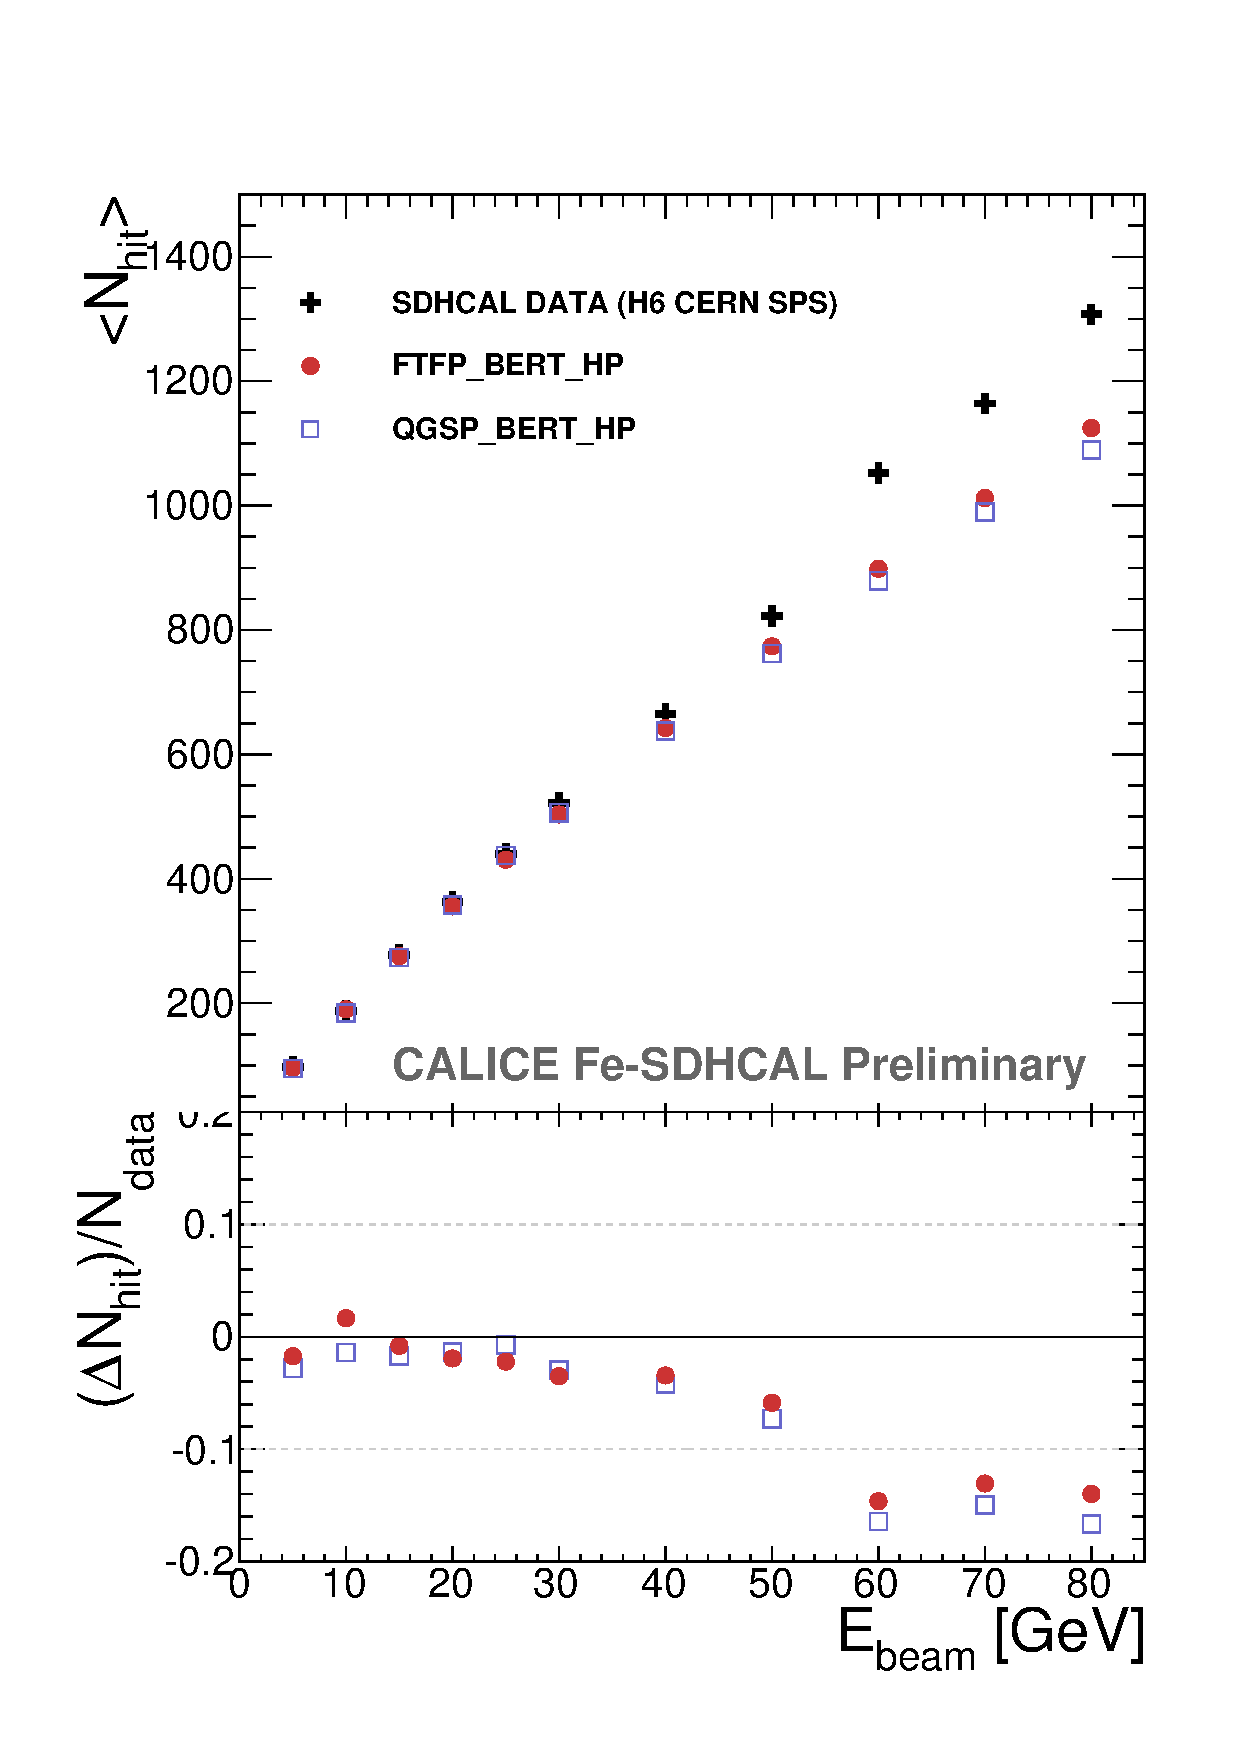
\includegraphics[width=.6\textwidth]{SDHCAL/figs/NHITPION.pdf}
    \caption{(a) Nombre moyen de coups en fonction de l'énergie du faisceau. La courbe noire pleine est un ajustement linéaire fait entre 5 et 20 $GeV$. La courbe noire en pointillé prolonge cet ajustement. (b) Déviation relative du nombre moyen de coups à l'ajustement linéaire en fonction de l'énergie du faisceau.}
    \label{fig:nhitLin}
  \end{center}
\end{figure}
Cette courbe est ajustée avec une fonction linéaire sur la gamme [0,20] $GeV$ (courbe noire trait plein). Cette courbe est prolongé sur toute la gamme d'énergie (courbe noire en pointillé). Cette figure présente aussi la déviation relative définie par $\frac{<N_{Hit}>-N_{Fit}}{N_{Fit}}$, où $<N_{Hit}>$ est le nombre moyen de coups et $N_{Fit}$ le nombre de coups attendus en utilisant le résultats de l'ajustement. Le nombre de coups dans le SDHCAL suit assez bien une fonction linéaire jusque 20 $GeV$. Au delà de 25 $GeV$, on remarque que la réponse du SDHCAL sature avec l'énergie. À 60 $GeV$, le nombre de coups remonte brusquement. Ceci est probablement dus à la contamination par les protons qui ont une longueur d'intéraction plus faible que celle des pions.
\begin{figure}[!h]
  \begin{center}
    \includegraphics[width=.7\textwidth]{SDHCAL/figs/Nhit_N1_N2_N3.pdf}
    \caption{Nombre moyen de coups pour chaque seuil en fonction de l'énergie du faisceau. Les cercles noires représentes le nombre de coups total. Les carrés verts représentent le nombre de coups pour le seuils 1. Les triangles bleus représentent le nombre de coups pour le seuils 2. Les croix rouges représentent le nombre de coups pour le seuils 3.}
    \label{fig:nhit123}
  \end{center}
\end{figure}
La figure~\ref{fig:nhit123} présente le nombre de coups moyen pour chaque seuil, en fonction de l'énergie du hadron incident. L'utilisation des seuils permettra de corriger l'effet de la saturation vu sur la figure~\ref{fig:nhitLin} afin d'améliorer la résolution en énergie.

\subsubsection{Le mode binaire}
Une première méthode pour reconstruire l'énergie des particules incidentes utilise uniquement le nombre de coups de chaque événement. L'énergie est mesurée en grâce à l'équation suivante:
\begin{equation}
  E_{reco} = A \cdot N_{Hit}
\end{equation}
où $A$ est une constante déterminée avec les données expérimentales. Cependant, la saturation observée sur la figure~\ref{fig:nhitLin} ne permet pas d'obtenir une linéarité satisfaisante au dessus de 30 $GeV$. Pour restaurer la linéarité, plusieurs paramétrisations ont été testé. La paramétrisation permettant d'obtenir une linéarité raisonnable est donnée par l'équation suivante:
\begin{equation}
  E_{reco} = A \cdot N_{Hit} + B \cdot N_{Hit}^2 + C \cdot N_{Hit}^3
\end{equation}
Les constantes $A$, $B$ et $C$ sont déterminées avec les données expérimentales en minimisant le $\chi^2$ suivant:
\begin{equation}
  \chi^2 = \frac{\sum_{i=0}^{N_{events}}(E_{inc}^i-E_{reco}^i)^2}{E_{inc}^i}
\end{equation}
où $N_{events}$ est le nombre d'événements utilisés pour la minimisation et $E_{inc}^i$ est l'énergie de la particule incidente $i$. La figure~\ref{fig:energy_dist_bin} montre deux distributions d'énergie reconstruite pour des échantillons de données à 20 et 40 $GeV$. 
\begin{figure}[!h]
  \begin{center}
    \includegraphics[width=.45\textwidth]{SDHCAL/figs/gfit-en-20-bin.pdf}
    \includegraphics[width=.45\textwidth]{SDHCAL/figs/gfit-en-40-bin.pdf}
    \caption{Distribution en énergie des gerbes hadroniques reconstruites. L'énergie est calculée avec le mode binaire sans l'information des seuils. Les distributions sont ajustés avec des gaussiennes dans une gamme de $\pm1.5\sigma$ autour de la valeur moyenne.}
    \label{fig:energy_dist_bin}
  \end{center}
\end{figure}
Les distributions d'énergie sont ajustées en deux temps, avec une fonction gaussienne. La valeur moyenne $\bar{E}_{reco}$ et le $\sigma$ d'un premier ajustement définissent la gamme [$\bar{E}_{reco}-1.5\sigma$ , $\bar{E}_{reco}+1.5\sigma$] pour le second ajustement. Cette méthode d'ajustement permet de s'affranchir des queues de distribution à basse énergie (à gauche sur les figures de distribution en énergie). Ces queues de distribution sont dus aux hadrons qui interagissent tardivement dans le détecteur. Ainsi, une fraction importante de l'énergie incidente n'est pas déposée dans le détecteur et détériore la reconstruction de l'énergie. La figure~\ref{fig:energy_bin}(a) montre le nombre moyen de coups et la déviation relative en fonction de l'énergie du faisceau. La déviation relative est définie par $\frac{E_{reco}-E_{beam}}{E_{beam}}$ ($E_{beam}$ est l'énergie du faisceau). Cette figure montre une très bonne linéarité ($\frac{E_{reco}-E_{beam}}{E_{beam}}<5\%$ sur toute la gamme d'énergie sauf à 5 $GeV$), ce qui valide le choix de la paramétrisation de $E_{reco}$.
\begin{figure}[!h]
  \begin{center}
    \subfigure[]{\includegraphics[width=.44\textwidth]{SDHCAL/figs/LINEARITY_bin_10.pdf}}
    \subfigure[]{\includegraphics[width=.55\textwidth]{SDHCAL/figs/RESO_bin_10.pdf}}
    \caption{(a): Énergie reconstruite moyenne des gerbes hadroniques et déviation relative en fonction de l'énergie de la particule incidente. (b): Résolution relative ($\frac{\sigma_{reco}}{E_{reco}}$) de l'énergie reconstruite en fonction de l'énergie du faisceau. L'énergie est calculée en utilisant uniquement le nombre total de coups.}
    \label{fig:energy_bin}
  \end{center}
\end{figure}
La figure~\ref{fig:energy_bin}(b) montre la résolution relative en fonction de l'énergie du faisceau.

\subsubsection{Le mode multi-seuils}
La spécificité du SDHCAL est son mode de lecture semi-digitale. Comme nous l'avons déjà expliqué, le seuil déclenché permet d'avoir une idée du nombre de particules secondaires traversant la couche de gaz vers un canal de lecture. Les informations sur les seuils devraient aider à combattre le phénomène de saturation vu sur la figure~\ref{fig:nhitLin} et à améliorer la résolution en énergie. Les informations des seuils pourraient aussi aider à comprendre la structure des gerbes hadroniques en identifiant les zones denses en particules secondaires. Une première tentative pour calculer l'énergie reconstruite des gerbes hadroniques utilisait:
\begin{equation}
  E_{reco}=\alpha\cdot N1+\beta\cdot N2+\gamma\cdot N3
  \label{eq.erec}
\end{equation}
avec $\alpha$, $\beta$ et $\gamma$ des constantes déterminées avec les données. Cependant, il s'est avéré impossible de trouver une paramétrisation de ces constantes donnant une bonne linéarité et une bonne résolution en énergie. Ainsi, comme pour le mode binaire, les paramètres de reconstruction de l'énergie sont des fonctions du nombre de coups total. La meilleurs paramétrisation obtenue est une fonction quadratique du nombre de coups (exemple:~$\alpha~=~A_1+B_1\cdot~N_{Hit}+C_1\cdot~N_{Hit}^2$). De même que pour le mode binaire, les valeurs des paramètres de l'énergie reconstruite sont déterminés avec une méthode de minimisation d'un $\chi^2$. 
\begin{figure}[!h]
  \begin{center}
    \includegraphics[width=.6\textwidth]{SDHCAL/figs/evolution.pdf}
    \caption{Évolution des paramètres de reconstruction de l'énergie en fonction du nombre total de coups. L'énergie est reconstruction en utilisant l'information des seuils.}
    \label{fig:evol}
  \end{center}
\end{figure}
La figure~\ref{fig:evol} montre l'évolution des paramètres de reconstruction de l'énergie en fonction du nombre total de coups. Le coefficient $\gamma$ (pour le troisième seuil) augmente avec le nombre de coups. Cela confirme l'idée que la présence des seuils aide à traiter le phénomène de saturation. La figure~\ref{fig:energy_dist_sd} montre deux distributions d'énergie reconstruite à 20 et 40 $GeV$ en utilisant la méthode multi-seuils. 
\begin{figure}[!h]
  \begin{center}
    \includegraphics[width=.45\textwidth]{SDHCAL/figs/gfit-en-20.pdf}
    \includegraphics[width=.45\textwidth]{SDHCAL/figs/gfit-en-40.pdf}
    \caption{Distribution en énergie des gerbes hadroniques reconstruites. L'énergie est calculée avec le mode multi-seuils. Les distributions sont ajustés avec des gaussiennes dans une gamme de $\pm1.5\sigma$ autour de la valeur moyenne.}
    \label{fig:energy_dist_sd}
  \end{center}
\end{figure}
De même que pour le mode binaire, les distribution d'énergie reconstruite sont ajustées en deux étapes avec une fonction gaussienne. 
\begin{figure}[!h]
  \begin{center}
    \subfigure[]{\includegraphics[width=.44\textwidth]{SDHCAL/figs/LINEARITY_Sept_10.pdf}}
    \subfigure[]{\includegraphics[width=.55\textwidth]{SDHCAL/figs/RESO_Sept_10.pdf}}
    \caption{(a): Énergie reconstruite moyenne des gerbes hadroniques et déviation relative en fonction de l'énergie de la particule incidente. (b): Résolution relative ($\frac{\sigma_{reco}}{E_{reco}}$) de l'énergie reconstruite en fonction de l'énergie du faisceau. L'énergie est calculée en utilisant le mode multi-seuils.}
    \label{fig:energy_sd}
  \end{center}
\end{figure}
La figure~\ref{fig:energy_sd}(a) présente la valeur moyenne de l'énergie reconstruite des gerbes hadroniques en fonction de l'énergie du faisceau en utilisant le mode multi-seuils. La déviation relative ($\frac{E_{reco}-E_{beam}}{E_{beam}}$) est en dessous de 5 $GeV$ sur toute la gamme d'énergie. La résolution relative ($\frac{\sigma_{reco}}{E_{reco}}$) est donnée par la figure~\ref{fig:energy_sd}(b). Cette résolution varie de 24$\%$ à 5 $GeV$ jusque 6.7$\%$ à 80 GeV. Ces résultats sont très encourageant et ont été obtenus sans corrections de gains qui devraient améliorer l'homogénéité de la réponse du SDHCAL. De plus, ces résultats ont été obtenus en utilisant uniquement le nombre de coups pour chaque seuil. Des méthodes utilisant de manière plus appropriée la très haute granularité du SDHCAL ont été développée. Nous avons déjà mentionné la méthode de Transformée de Hough (section~\ref{sec.pi_selection} de ce chapitre) pour identifié des traces dans les gerbes hadroniques. L'énergie déposée par les particules dans les traces est faible. La formule utilisée pour reconstruire (equation~\ref{eq.erec}) pourrait être adaptée afin de séparer la contribution des traces de reste de la gerbe hadroniques:
\begin{equation}
  E_{reco}=\alpha\cdot (N1-N1_{HT})+\beta\cdot (N2-N2_{HT})+\gamma\cdot (N3-N3_{HT}) + C\cdot(N1_{HT}+N2_{HT}+N3_{HT}) 
  \label{eq.erec_ht}
\end{equation}
où $N1_{HT}$, $N2_{HT}$ et $N3_{HT}$ correspondent au nombre de coups pour chaque seuils dans les traces et $C$ est une constante à déterminer avec les données expérimentales. De plus, dans ces traces, on retrouve des coups avec le seuil 2 ou 3 (voir figure~\ref{fig:shower80}). Ces coups ne correspondent pas forcément à une zone avec beaucoup de particules secondaires. Ils sont plutôt produits à cause de fluctuations de la charge induite de l'avalanche dans la couche de gaz. Nous verrons comment cette distribution de charge est extraite dans le chapitre~\ref{chap.simulation}. Une méthode de reconstruction de l'énergie identifiant la partie électromagnétique des gerbes hadroniques a aussi été testé. Les résultats obtenus sont comparables avec la méthode multi-seuils standard. 
\subsubsection{Comparaison du mode binaire et multi-seuils}
Deux méthode de reconstruction de l'énergie ont été présenté. La figure~\ref{fig:multi_vs_binary_dist} montre les distributions d'énergie reconstruite à 20 et 80 $GeV$ avec les deux méthodes (mode binaire et multi-seuils).
\begin{figure}[!h]
  \begin{center}
    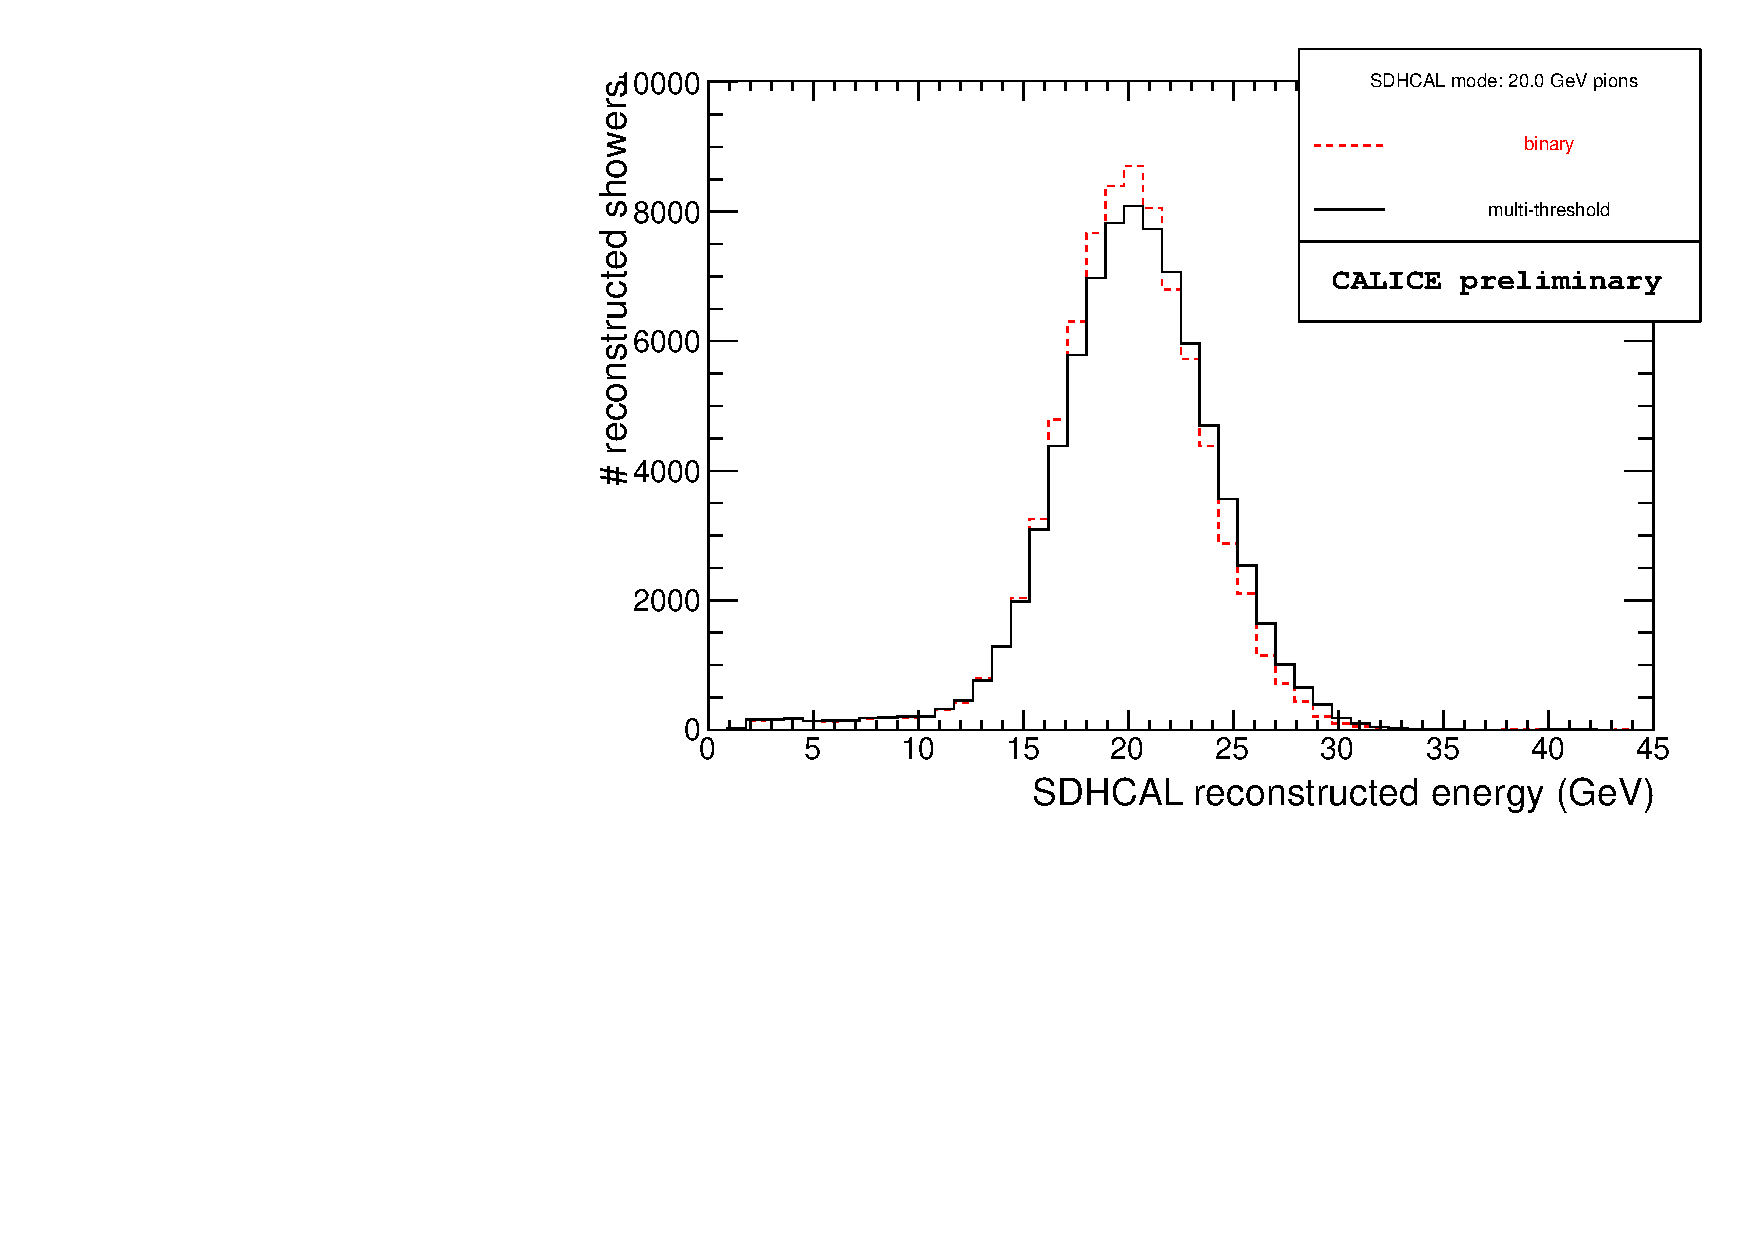
\includegraphics[width=.45\textwidth]{SDHCAL/figs/Pi20GeV_SDHCAL_2modes_overlay.pdf}
    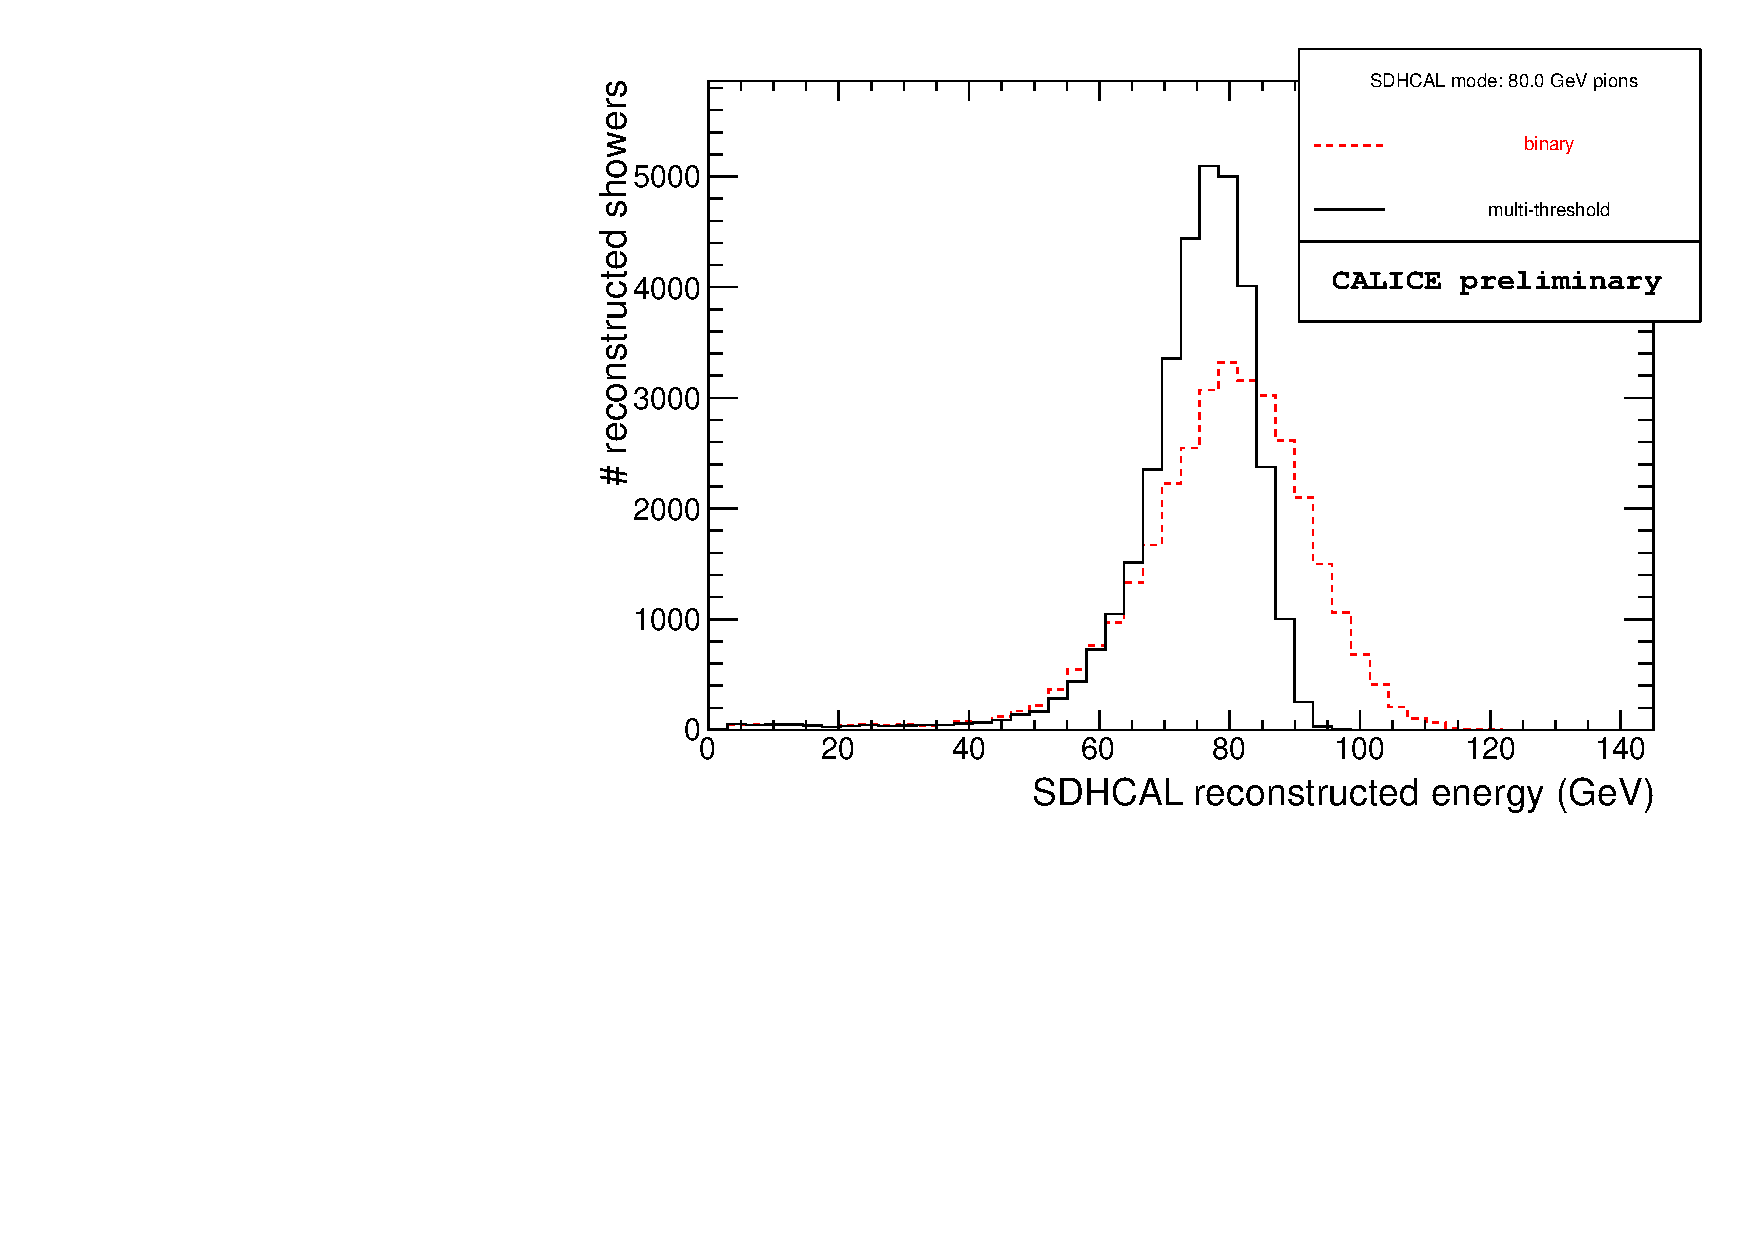
\includegraphics[width=.45\textwidth]{SDHCAL/figs/Pi80GeV_SDHCAL_2modes_overlay.pdf}
    \caption{Distribution d'énergie à 20 (à droite) et à 80 (à gauche) $GeV$ avec la méthode binaire (en pointillé rouge) et la méthode multi-seuils (trait plein).}
    \label{fig:multi_vs_binary_dist}
  \end{center}
\end{figure}
À $20$ GeV, la différence entre les deux méthodes est faible, avec même une distribution légèrement plus étroite pour le mode binaire. Cependant, à 80 $GeV$, la distribution d'énergie reconstruite avec la méthode multi-seuils est beaucoup plus étroites que celle reconstruite avec la méthode binaire. La figure~\ref{fig:multi_vs_binary_res} présente la résolution relative en fonction de l'énergie du faisceau pour les deux méthodes.
\begin{figure}[!h]
  \begin{center}
    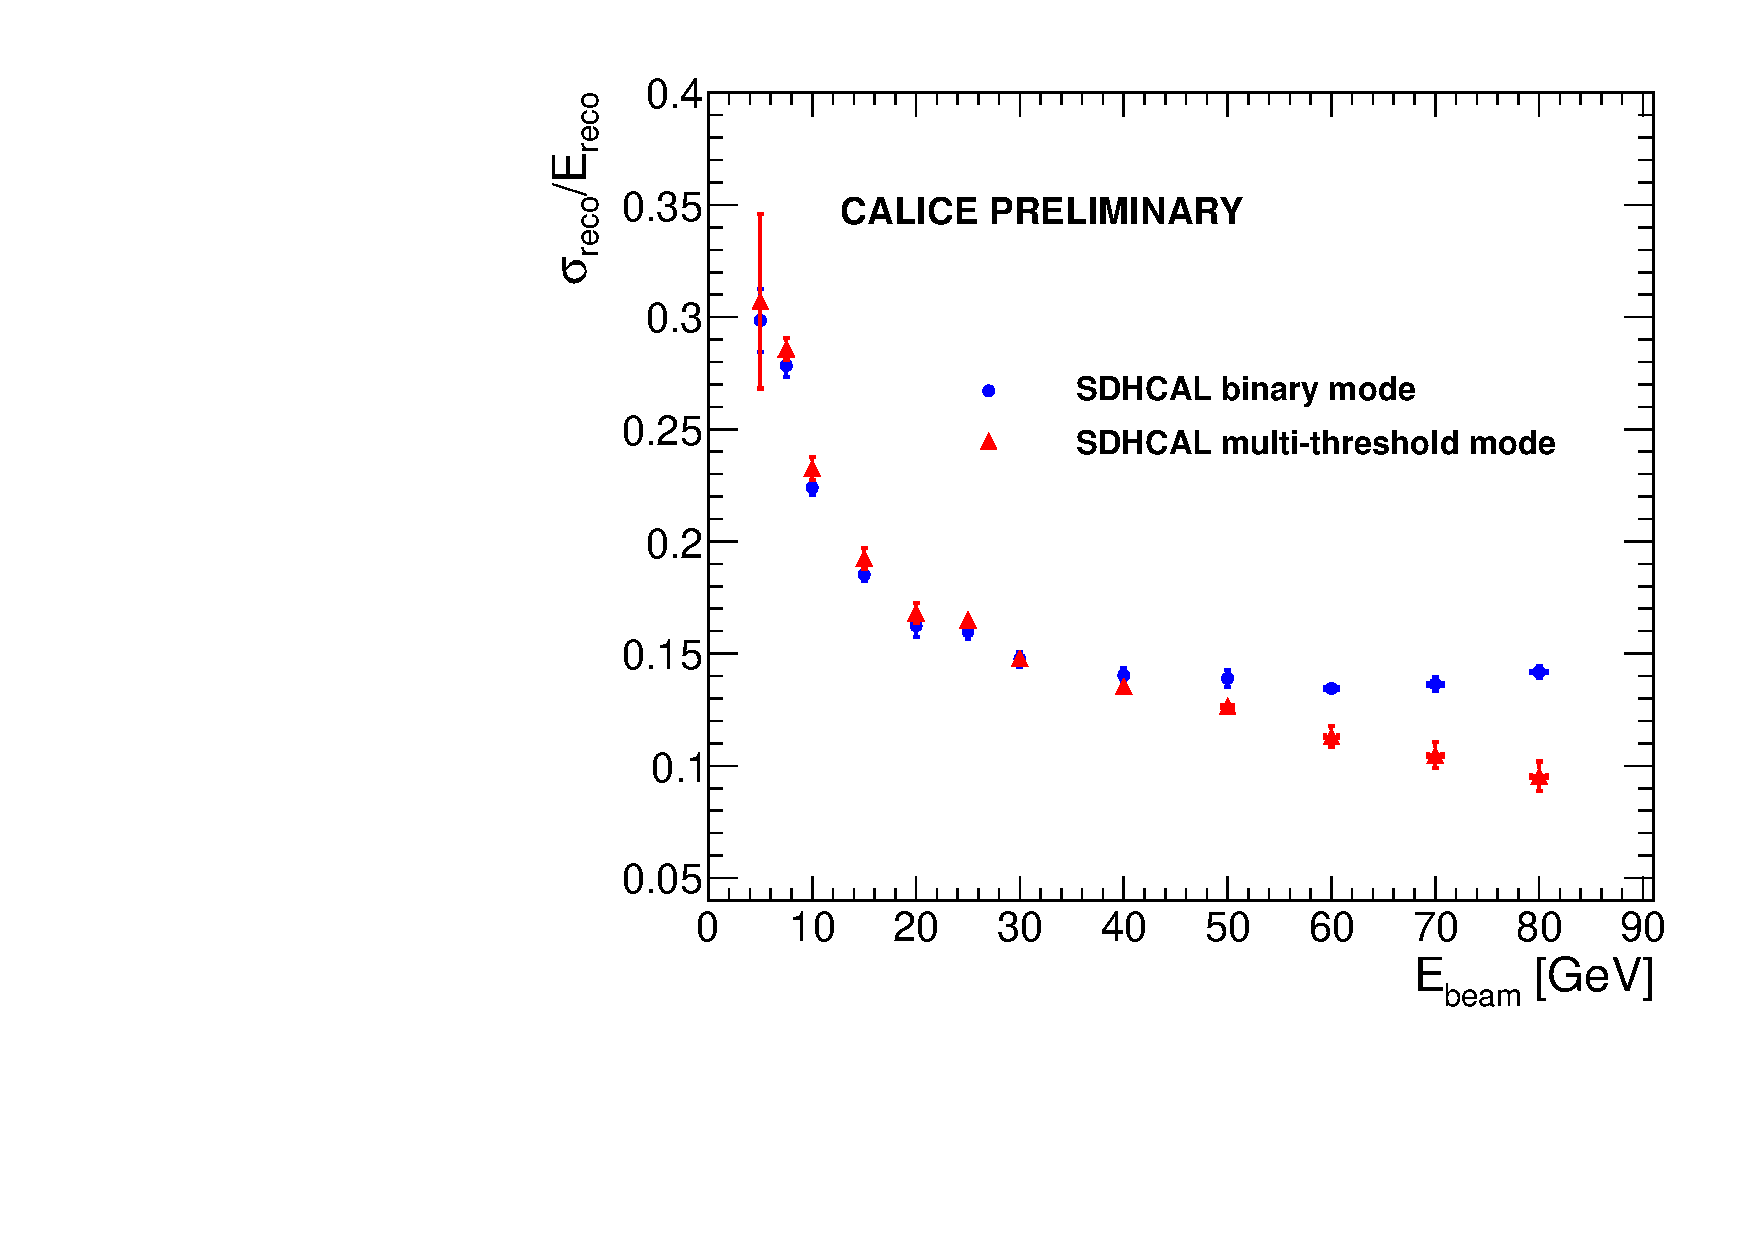
\includegraphics[width=.55\textwidth]{SDHCAL/figs/RESOLUTION.pdf}
    \caption{Résolution en énergie en fonction de l’énergie du faisceau pour le mode binaire et multi-seuils.}
    \label{fig:multi_vs_binary_res}
  \end{center}
\end{figure}
Jusque 30 $GeV$, les résolutions en énergie sont comparables pour les deux méthodes. Au dessus de 40 $GeV$, la résolution pour le mode multi-seuils est meilleurs. Cette comparaison permet de valider le concept du SDHCAL: la résolution en énergie obtenue avec un calorimètre hadronique gazeux ultra-granulaire est très satisfaisante et l'utilisation des seuils permet de lutter contre la saturation et ainsi d'améliorer la résolution en énergie.

\section{Performance du SDHCAL avec correction de gains}
\label{sec.gainCorrectRes}
